\documentclass{report}
\usepackage{vntex}
\usepackage[utf8]{inputenc}
\usepackage[unicode]{hyperref}
\usepackage{setspace}
\usepackage[a4paper,width=150mm,top=20mm,bottom=20mm,left=30mm,right=20mm]{geometry}
\usepackage{fancyhdr}
\usepackage{graphicx}
\usepackage{color}
\graphicspath{ {figures/} }
\usepackage{array}
\usepackage{float}
\usepackage{indentfirst}
\usepackage{enumerate}
\usepackage{makecell}
\usepackage[table]{xcolor}% http://ctan.org/pkg/xcolor
\usepackage{ifthen}
\usepackage{caption}
\usepackage{subcaption}
\usepackage{pdfpages}
\usepackage{minitoc}
\usepackage[toc,page,header]{appendix}
\usepackage{etoolbox}
\usepackage{longtable}
\usepackage{enumitem}


\setcounter{secnumdepth}{3}
\setcounter{tocdepth}{2}

\usepackage{titlesec}
\titleformat*{\subsubsection}{\fontsize{12pt}{12pt}\selectfont\bfseries}

\renewcommand{\chaptermark}[1]{\markboth{#1}{}}     % remove chapter number on header
\fancyhf{}                  % clear all header, footer
\fancyhead[L]{\leftmark}    % set header
\fancyfoot[C]{\thepage}     % set footer


\newcommand{\stoptocwriting}{%
  \addtocontents{toc}{\protect\setcounter{tocdepth}{-5}}}
\newcommand{\resumetocwriting}{%
  \addtocontents{toc}{\protect\setcounter{tocdepth}{\arabic{tocdepth}}}}




\appto\appendix{\addtocontents{toc}{\protect\setcounter{tocdepth}{0}}}
% reinstate the correct level for list of tables and figures
\appto\listoffigures{\addtocontents{lof}{\protect\setcounter{tocdepth}{1}}}
\appto\listoftables{\addtocontents{lot}{\protect\setcounter{tocdepth}{1}}}



% \renewcommand{\appendixtocname}{<Appendixx>}
% \addto\captionsitalian{%
%    \renewcommand{\appendixtocname}{Appendici}%
%    \renewcommand{\appendixpagename}{Appendici}%
% }



\usepackage{listings}
\usepackage{color}
\usepackage{listingsutf8}

\definecolor{dkgreen}{rgb}{0,0.6,0}
\definecolor{gray}{rgb}{0.5,0.5,0.5}
\definecolor{mauve}{rgb}{0.58,0,0.82}

% Define Javascript language
\lstdefinelanguage{JavaScript}{
  keywords={typeof, new, true, false, catch, function, return, null, catch, switch, var, if, in, while, do, else, case, break},
  keywordstyle=\color{blue}\bfseries,
  ndkeywords={class, export, boolean, throw, implements, import, this},
  ndkeywordstyle=\color{darkgray}\bfseries,
  identifierstyle=\color{black},
  sensitive=false,
  comment=[l]{//},
  morecomment=[s]{/*}{*/},
  commentstyle=\color{purple}\ttfamily,
  stringstyle=\color{red}\ttfamily,
  morestring=[b]',
  morestring=[b]"
}

\lstset{
  language=JavaScript,
  backgroundcolor=\color{lightgray},
  extendedchars=true,
  basicstyle=\footnotesize\ttfamily,
  showstringspaces=false,
  showspaces=false,
  numbers=left,
  numberstyle=\footnotesize,
  numbersep=9pt,
  tabsize=2,
  breaklines=true,
  showtabs=false,
  captionpos=b
}

% Define language terraform - kubernetes
\lstdefinelanguage{terraform}{
  keywords={terraform, variable, locals, output, module, resource, data, provider, lifecycle, provisioner, connection, count, for_each, depends_on, provider, for, if, metadata, spec, type},
  backgroundcolor=\color{white},
  keywordstyle=\color{blue}\bfseries,
  identifierstyle=\color{black},
  sensitive=false,
  comment=[l]{\#},
  commentstyle=\color{gray}\ttfamily,
  stringstyle=\color{purple}\ttfamily,
  morestring=[b]',
  morestring=[b]"
}


\lstset{basicstyle=\ttfamily,
  showstringspaces=false,
  commentstyle=\color{red},
  keywordstyle=\color{blue},
  inputencoding=utf8,
  extendedchars=true
}


\lstset{frame=tb,
  language=Java,
  aboveskip=3mm,
  belowskip=3mm,
  showstringspaces=false,
  columns=flexible,
  basicstyle={\small\ttfamily},
  numbers=none,
  numberstyle=\tiny\color{gray},
  keywordstyle=\color{blue},
  commentstyle=\color{dkgreen},
  stringstyle=\color{mauve},
  breaklines=true,
  breakatwhitespace=true,
  tabsize=3
}

% \renewcommand{\lstlistingname}{Mã nguồn}
% \renewcommand{\lstlistlistingname}{Danh sách mã nguồn}
% Docker syntax highlight
\lstdefinelanguage{docker}{
  keywords={FROM, RUN, COPY, ADD, ENTRYPOINT, CMD,  ENV, ARG, WORKDIR, EXPOSE, LABEL, USER, VOLUME, STOPSIGNAL, ONBUILD, MAINTAINER},
  backgroundcolor=\color{white},
  keywordstyle=\color{blue}\bfseries,
  identifierstyle=\color{black},
  sensitive=false,
  comment=[l]{\#},
  commentstyle=\color{purple}\ttfamily,
  stringstyle=\color{red}\ttfamily,
  morestring=[b]',
  morestring=[b]"
}

\lstdefinelanguage{docker-compose}{
  keywords={image, environment, ports, container_name, ports, volumes, links},
  keywordstyle=\color{blue}\bfseries,
  identifierstyle=\color{black},
  sensitive=false,
  comment=[l]{\#},
  commentstyle=\color{purple}\ttfamily,
  stringstyle=\color{red}\ttfamily,
  morestring=[b]',
  morestring=[b]"
}
\lstdefinelanguage{docker-compose-2}{
  % keywords={version, volumes, services},
  keywords={image, environment, ports, container_name, ports, volumes, links, working_dir, command, networks, services, restart, build, context, dockerfile, depends_on},
  keywordstyle=\color{blue}\bfseries,
  % keywords=[10]{sfu:, controller:, mongodb:, message-broker-server, event-simulator, node-api-server, node-api-gateway, redis},
  % keywordstyle=[10]\color{olive}\bfseries,
  identifierstyle=\color{black},
  sensitive=false,
  comment=[l]{\#},
  commentstyle=\color{purple}\ttfamily,
  stringstyle=\color{red}\ttfamily,
  morestring=[b]',
  morestring=[b]"
}

%%%%%%%%%%%%%%%%%%%%%%%%%%%%%%%%%%%%%%%%%%%%%%%%%%%%%%
%%%%%%%%%%% YAML syntax highlighting %%%%%%%%%%%%%%%%%

% http://tex.stackexchange.com/questions/152829/how-can-i-highlight-yaml-code-in-a-pretty-way-with-listings

% here is a macro expanding to the name of the language
% (handy if you decide to change it further down the road)
\newcommand\YAMLcolonstyle{\color{red}\mdseries}
\newcommand\YAMLkeystyle{\color{black}\bfseries}
\newcommand\YAMLvaluestyle{\color{blue}\mdseries}

\makeatletter

\newcommand\language@yaml{yaml}

\expandafter\expandafter\expandafter\lstdefinelanguage
\expandafter{\language@yaml}
{
  keywords={true,false,null,y,n},
  % assuming a key comes first
  backgroundcolor=\color{white}
  sensitive=false,
  comment=[l]{\#},
  morecomment=[s]{/*}{*/},
  commentstyle=\color{purple}\ttfamily,
  stringstyle=\YAMLvaluestyle\ttfamily,
  moredelim=[l][\color{orange}]{\&},
  moredelim=[l][\color{magenta}]{*},
  moredelim=**[il][\YAMLcolonstyle{:}\YAMLvaluestyle]{:},   % switch to value style at :
  morestring=[b]',
  morestring=[b]",
  literate =    {---}{{\ProcessThreeDashes}}3
                {>}{{\textcolor{red}\textgreater}}1     
                {|}{{\textcolor{red}\textbar}}1 
                {\ -\ }{{\mdseries\ -\ }}3,
}

% switch to key style at EOL
\lst@AddToHook{EveryLine}{\ifx\lst@language\language@yaml\YAMLkeystyle\fi}
\makeatother

\newcommand\ProcessThreeDashes{\llap{\color{cyan}\mdseries-{-}-}}

%%%%%%%%%%% YAML syntax highlighting %%%%%%%%%%%%%%%%%
%%%%%%%%%%%%%%%%%%%%%%%%%%%%%%%%%%%%%%%%%%%%%%%%%%%%%%

\onehalfspacing
\begin{document}

\begingroup
\fontsize{12pt}{12pt}\selectfont

%%%%%%%%%%%%%%%%%%%%% LVTN %%%%%%%%%%%%%%%%%%%%%
% \newpage
% \thispagestyle{empty}
% % Phiếu nhiệm vụ
% \includepdf[pages={1}]{pdf/phieunhiemvu.pdf}
% \newpage
% \thispagestyle{empty}
% % Phiếu chấm hướng dẫn
% \includepdf[pages=-]{pdf/phieuchamhuongdan.pdf}
% \newpage
% \thispagestyle{empty}
% % Phiếu phản biện
% \includepdf[pages=-]{pdf/phieuchamphanbien.pdf}

% \newpage
% % \includepdf[pages=-]{pdf/cover.pdf}
% \includepdf[pages=-]{pdf/cover_GD2 - final - Copy.pdf}


% \newpage
% \thispagestyle{empty}
% % Phiếu nhiệm vụ
% \includepdf[pages={1}]{pdf/phieunhiemvu.pdf}
% \newpage
% \thispagestyle{empty}
% % Phiếu chấm hướng dẫn
% \includepdf[pages=-]{pdf/phieuchamhuongdan.pdf}
% \newpage
% \thispagestyle{empty}
% % Phiếu phản biện
% \includepdf[pages=-]{pdf/phieuchamphanbien.pdf}

% \newpage
% \thispagestyle{empty}
% \input{sections/signatures}

\pagenumbering{roman}
\newpage
\begin{titlepage}

    \begingroup
        \fontsize{15pt}{12pt}\selectfont
        \begin{center}
            \textbf{
                ĐẠI HỌC QUỐC GIA THÀNH PHỐ HỒ CHÍ MINH \\
                TRƯỜNG ĐẠI HỌC BÁCH KHOA \\
                KHOA KHOA HỌC VÀ KỸ THUẬT MÁY TÍNH
            }
        \end{center}       
    \endgroup
    
    \vspace{1cm}
    
    \begin{figure}[h!]
        \begin{center}
            
\includegraphics[width=4cm]{images/hcmut.png}
        \end{center}
    \end{figure}
    
    \vspace{0.5cm}

    \begingroup
        \fontsize{15pt}{12pt}\selectfont
        \begin{center}
            \textbf{BÁO CÁO} \\
            \textbf{ĐỒ ÁN CHUYÊN NGÀNH}
        \end{center}       
    \endgroup

    \vspace{0.5cm}


    \begingroup
        \fontsize{18pt}{12pt}\selectfont
        \begin{center}
            \textbf{PHÁT TRIỂN HỆ THỐNG THƯƠNG MẠI ĐIỆN TỬ CÓ TÍNH SẴN SÀNG VÀ MỞ RỘNG CAO CHO SẢN PHẨM CÔNG NGHỆ}
        \end{center}       
    \endgroup

    \vspace{0.5cm}

    \begingroup
        \fontsize{15pt}{12pt}\selectfont
        \begin{center}
            Ngành: Khoa học Máy tính
        \end{center}       
    \endgroup
    
    \vspace{1.5cm}

    \begingroup
        \fontsize{14pt}{12pt}\selectfont
        \begin{center}
            \begin{tabular}{rll}
                \color{black} \textbf{Hội đồng:} & \color{black} Đồ án chuyên ngành &  \\
                \color{black} \textbf{Giảng viên hướng dẫn:} & \color{black} Phan Trọng Nhân &  \\

                \\

                \multicolumn{3}{c}{\noindent\rule{4cm}{0.5pt} \textbf{oOo} \noindent\rule{4cm}{0.5pt}} \\ \\
                \color{black}\textbf{Sinh viên thực hiện 1:} & \color{black}Lê Hoàng Anh & \color{black}1910752 \\
                \color{black}\textbf{Sinh viên thực hiện 2:} & \color{black}Hoàng Văn Hiếu & \color{black}1913328 \\
                \color{black}\textbf{Sinh viên thực hiện 3:} & \color{black}Thới Duy Phát & \color{black}2120049 \\
            \end{tabular}
        \end{center}
    \endgroup
    
    \vspace{1.5cm}

    \begingroup
        \fontsize{12pt}{12pt}\selectfont
        \begin{center}
            {TP. Hồ Chí Minh, Tháng 12/2023}
        \end{center}
    \endgroup
    
\end{titlepage}

\newpage
\tableofcontents

\newpage
\thispagestyle{empty}
\listoftables
\listoffigures
% \lstlistoflistings

\newpage

\pagestyle{fancy}



\pagenumbering{arabic}
\chapter{Giới thiệu}
% \section{Ví dụ}

% \noindent Đây là một ví dụ, sau này sẽ được update nội dung sau.

% If this chapter/section has a star, it won't be in the table of content.
% \section*{Đây là section k dc thêm vào mục lục}
\section{Giới thiệu đề tài}
\noindent Trong thời đại công nghệ số và đại dịch, việc mua sắm trực tuyến đang trở nên phổ biến hơn bao giờ hết. Điều này đặt ra một thách thức lớn cho các doanh nghiệp, đòi hỏi họ phải sở hữu kênh bán hàng trực tuyến để đáp ứng nhu cầu của khách hàng. Đề tài này nhằm xây dựng một hệ thống thương mại điện tử linh hoạt, ổn định và có khả năng mở rộng trên nhiều nền tảng khác nhau. Hệ thống này cũng phải dễ dàng bảo trì và nâng cấp trong tương lai. Do đó, việc một doanh nghiệp sở hữu kênh bán hàng trên nền tảng số là vô cùng cần thiết. Mục tiêu của đề tài là xây dựng một hệ thống thương mại điện tử có tính sẵn sàng, tính mở rộng cao, có thể được đưa lên nhiều nền tảng khác nhau một cách dễ dàng, dễ bảo trì, nâng cấp trong tương lai.

\section{Mục tiêu và phạm vi của đề tài}
\noindent Hệ thống bao gồm những chức năng chính cho một trang web thương mại điện tử bán sản phẩm công nghệ và một số tính năng, đặc điểm nổi bật như tính sẵn sàng cao, tính mở rộng cao, đáp ứng được lưu lượng truy cập biến động của người dùng.

\section{Cấu trúc đồ án}
\noindent Nội dung của đồ án được trình bày bao gồm những chương sau
% {\renewcommand\labelitemi{}
% \begin{itemize}
%     \item Chương I Giới thiệu chung về đề tài
%     \item Chương II Cơ sở lý thuyết
%     \item Chương III Tổng hợp và phân tích bài toán
%     \item Chương IV Thiết kế hệ thống
%     \item Chương V Xây dựng phiên bản thử nghiệm
% \end{itemize}
% }

\begin{enumerate}[label=\Roman*., itemsep=0pt, start=1]
    \item Giới thiệu chung về đề tài
    \item Cơ sở lý thuyết
    \item Tổng hợp và phân tích bài toán
    \item Thiết kế hệ thống
    \item Xây dựng phiên bản thử nghiệm
\end{enumerate}
\chapter{Cơ sở lý thuyết}
\section{Các cơ sở lý thuyết và công nghệ sử dụng}
\subsection{Reactjs}
\subsubsection{Khái niệm}
\indent ReactJS là một thư viện JavaScript phía người dùng (frontend) được sử dụng để xây dựng giao diện người dùng tương tác \footnote{https://fptcloud.com/reactjs/}.
\subsubsection{Ưu điểm của Reactjs}
\begin{itemize}
    \item \textbf{Tận dụng lại các thành phần có sẵn}

    \indent ReactJS hỗ trợ tích cực trong khởi tạo một website bởi lập trình viên sẽ không cần phải code nhiều như khi tạo trang web mà chỉ sử dụng JavaScript. Đồng thời, nó cung cấp một loạt các thành phần sẵn có mà bạn có thể sử dụng trong nhiều tình huống khác nhau.
    \item \textbf{Tích hợp được cho cả ứng dụng di động Mobile application}

    \indent Hầu hết chúng ta đã biết rằng ReactJS được sử dụng để phát triển các ứng dụng web, tuy nhiên, nó không chỉ giới hạn trong lĩnh vực đó. Nếu chúng ta muốn phát triển các ứng dụng di động, chúng ta có thể sử dụng React Native. Đây là một framework do Facebook phát triển, cho phép chúng ta dễ dàng "chia sẻ" các thành phần và tái sử dụng logic nghiệp vụ trong các ứng dụng của chúng ta.
    \item \textbf{Tối ưu để tăng cường khả năng tìm kiếm SEO}

    \indent Tối ưu hóa công cụ tìm kiếm (SEO) là một yếu tố quan trọng để đảm bảo trang web của chúng ta xuất hiện cao hơn trong kết quả tìm kiếm của Google. ReactJS là một thư viện JavaScript cơ bản. Công cụ tìm kiếm của Google có khả năng thu thập thông tin và lập chỉ mục mã JavaScript, tuy nhiên, nó cũng yêu cầu sự hỗ trợ từ các thư viện khác để làm điều này.
    \item \textbf{Dễ dàng sửa lỗi và gỡ rối Debug}

    \indent Facebook đã phát hành một tiện ích mở rộng Chrome để hỗ trợ việc gỡ lỗi trong quá trình phát triển ứng dụng. Điều này giúp tăng tốc quá trình phát hành sản phẩm cũng như quá trình viết mã của chúng ta.
\end{itemize}
\subsubsection{Nhược điểm của Reactjs}
\begin{itemize}
    \item Reactjs không phải là framework, cho nên chúng ta phải tự xây dựng dự án bằng thủ công.
    \item Tích hợp Reactjs vào các framework MVC truyền thống yêu cầu cần phải cấu hình lại.
    \item Poor Document: Đó là một nhược điểm khá phổ biến đối với các công nghệ cập nhật liên tục. Các công nghệ cập nhật và tăng tốc nhanh đến mức không có thời gian để tạo tài liệu phù hợp.
\end{itemize}
\subsection{Java Spring Boot}

\subsubsection{Khái niệm} Spring Boot là một framework phát triển ứng dụng Java, dựa trên nền tảng Spring Framework. Nó được thiết kế để giảm bớt công việc cấu hình và cung cấp một cách tiếp cận linh hoạt và nhanh chóng để xây dựng các ứng dụng Java.\footnote{https://lotusacademy.edu.vn/blog/java-spring-boot-la-gi-java-spring-mvc-la-gi-spring-framework-la-gi-256}

\subsubsection{Ưu điểm}
\begin{itemize}
    \item \textbf{Tự động cấu hình:} Spring Boot tự động cấu hình dựa trên các quy tắc mặc định và cung cấp một số cấu hình tùy chỉnh đơn giản.
    \item \textbf{Tiết kiệm thời gian:} Với Spring Boot, bạn không cần lo lắng về việc cấu hình chi tiết và tập trung vào việc phát triển chức năng của ứng dụng.
    \item \textbf{Tích hợp dễ dàng:} Spring Boot tích hợp tốt với các công nghệ và thư viện phổ biến khác, cho phép bạn dễ dàng tích hợp các thành phần khác như cơ sở dữ liệu, bảo mật, gửi email, vv.
    \item \textbf{Gói hóa ứng dụng:} Spring Boot cho phép bạn gói hóa ứng dụng thành file JAR hoặc WAR, giúp dễ dàng triển khai và chạy trên các môi trường khác nhau.
\end{itemize}

\subsubsection{Nhược điểm}
\begin{itemize}
    \item \textbf{Phụ thuộc:} Spring Boot có thể tạo ra các ứng dụng có phụ thuộc tăng cao vào framework, điều này có thể làm cho ứng dụng phải dựa vào các phiên bản và cấu hình cụ thể của Spring Boot.
    \item \textbf{Tính linh hoạt:} Mặc dù Spring Boot giảm bớt công việc cấu hình, nhưng đôi khi nó có thể hạn chế tính linh hoạt so với việc cấu hình thủ công bằng XML hoặc Java.
    \item \textbf{Độ phức tạp:} Một số tính năng và cấu hình cao cấp của Spring Boot có thể trở nên phức tạp và khó hiểu đối với những người mới sử dụng.
\end{itemize}
\indent Tuy nhiên, ưu điểm của Spring Boot thường vượt trội hơn so với nhược điểm, vì nó giúp đơn giản hóa việc phát triển và triển khai ứng dụng Java.

\subsection{Nodejs}
\subsubsection{Khái niệm}
\indent Node.js là một môi trường chạy mã JavaScript phía máy chủ, dựa trên JavaScript Engine V8 của Google. Nó cho phép viết mã JavaScript để xây dựng ứng dụng máy chủ một cách hiệu quả. \footnote{https://nodejs.org/en/about}
\subsubsection{Ưu điểm của Node.js}
\begin{itemize}
    \item Hiệu suất cao: Với JavaScript Engine V8 nhanh chóng, Node.js cho phép xử lý các yêu cầu đồng thời một cách hiệu quả và đạt được hiệu suất cao.
    \item Đơn luồng và không đồng bộ: Node.js sử dụng mô hình xử lý không đồng bộ (non-blocking) I/O, giúp xử lý nhiều yêu cầu cùng một lúc mà không tốn thêm tài nguyên.
    \item Quản lý gói dễ dàng: Node.js có npm (Node Package Manager), cung cấp một kho lưu trữ gói phong phú và dễ quản lý.
    \item Phát triển đồng nhất: Với Node.js, phát triển ứng dụng web và ứng dụng di động có thể được thực hiện bằng cùng một ngôn ngữ và công cụ, tạo sự đồng nhất.
\end{itemize}
\subsubsection{Nhược điểm của Node.js}
\begin{itemize}
    \item Chưa phù hợp cho các tác vụ nặng: Do Node.js sử dụng mô hình đơn luồng, nó không phù hợp cho các tác vụ tính toán nặng hoặc xử lý dữ liệu lớn.
    \item Đòi hỏi khéo léo trong việc quản lý bộ nhớ: Node.js không tự động quản lý bộ nhớ, điều này yêu cầu phải làm việc thủ công để tránh rò rỉ bộ nhớ.
\end{itemize}
\subsection{Docker}
\subsubsection{Khái niệm}
\indent Docker là một nền tảng mã nguồn mở giúp đóng gói các ứng dụng và các phụ thuộc của chúng vào những đơn vị gọi là containers. Containers cho phép triển khai một ứng dụng một cách đáng tin cậy và di động với sự độc lập về môi trường.\footnote{https://docs.docker.com/}
\subsubsection{Ưu điểm}
\begin{itemize}
    \item Đóng gói và triển khai dễ dàng: Docker giúp đóng gói các ứng dụng và phụ thuộc vào một container có thể di chuyển được và triển khai một cách dễ dàng trên nhiều môi trường khác nhau.
    \item Tính nhất quán giữa môi trường phát triển và triển khai: Docker đảm bảo môi trường chạy ứng dụng trên máy chủ phát triển giống với môi trường chạy trên môi trường triển khai.
    \item Hiệu suất cao: Containers Docker nhẹ và nhanh chóng, giúp tối ưu hóa tài nguyên và cung cấp hiệu suất cao cho các ứng dụng.
\end{itemize}
\subsubsection{Nhược điểm}
\begin{itemize}
    \item Tăng phức tạp: Đôi khi quản lý các container Docker và xử lý các phụ thuộc có thể trở nên phức tạp, đặc biệt là trong các môi trường lớn và phức tạp.
    \item Hiệu suất ảnh hưởng: Mặc dù Docker giúp tối ưu hóa hiệu suất, nhưng việc sử dụng container cũng có thể ảnh hưởng đến hiệu suất so với việc chạy ứng dụng trực tiếp trên máy chủ vật lý.
\end{itemize}

\subsection{Terraform}
\subsubsection{Khái niệm}
\indent Terraform là một công cụ mã hóa cấu hình (Infrastructure as Code) được sử dụng để tự động hóa việc triển khai và quản lý cơ sở hạ tầng đám mây và hạ tầng điện toán.\footnote{https://www.alibabacloud.com/blog/terraform}
\subsubsection{Ưu điểm}
\begin{itemize}
    \item Tự động hóa hạ tầng: 
    Terraform cho phép viết mã để mô tả và triển khai cơ sở hạ tầng một cách dễ dàng và nhất quán.
    \item Đa nền tảng: 
    Terraform hỗ trợ nhiều nhà cung cấp đám mây và nền tảng hạ tầng khác nhau như AWS, Azure, GCP, v.v., giúp quản lý và triển khai đồng nhất trên nhiều môi trường.
    \item Kiểm soát phiên bản: 
    Terraform quản lý các tài nguyên hạ tầng như mã nguồn, cho phép theo dõi và quản lý phiên bản tài nguyên trong quá trình phát triển và triển khai.
\end{itemize}
\subsubsection{Nhược điểm}
\begin{itemize}
    \item Học và quản lý đòi hỏi thời gian: Terraform có độ dốc học đôi khi khá lớn, và việc quản lý mã cấu hình có thể đòi hỏi thời gian và kỹ năng.
    \item Giới hạn của các nhà cung cấp đám mây: Các nhà cung cấp đám mây có thể không hỗ trợ tất cả các tính năng của Terraform hoặc có giới hạn trong việc quản lý hạ tầng.
\end{itemize}
\subsection{Kubernetes}
\subsubsection{Khái niệm}
\indent Kubernetes (thường được gọi là k8s) là một nền tảng mã nguồn mở để quản lý việc triển khai, tự động hóa và mở rộng ứng dụng container.\footnote{https://kubernetes.io/vi/docs/concepts/overview/what-is-kubernetes/}

\indent Các ứng dụng có sử dụng Kubernetes: Google, Netflix, Airbnb, Spotify, Grab, Zalando, Adidas...và nhiều hơn nữa. Kubernetes đã trở thành một công nghệ phổ biến và mạnh mẽ trong việc quản lý và triển khai ứng dụng quy mô lớn.
\subsubsection{Kiến trúc}
Hình ảnh được tham khảo từ bài viết "What Is Kubernetes Architecture? – Components Overview"\footnote{https://spacelift.io/blog/kubernetes-architecture}
 \begin{figure}[H]
    \begin{center}
    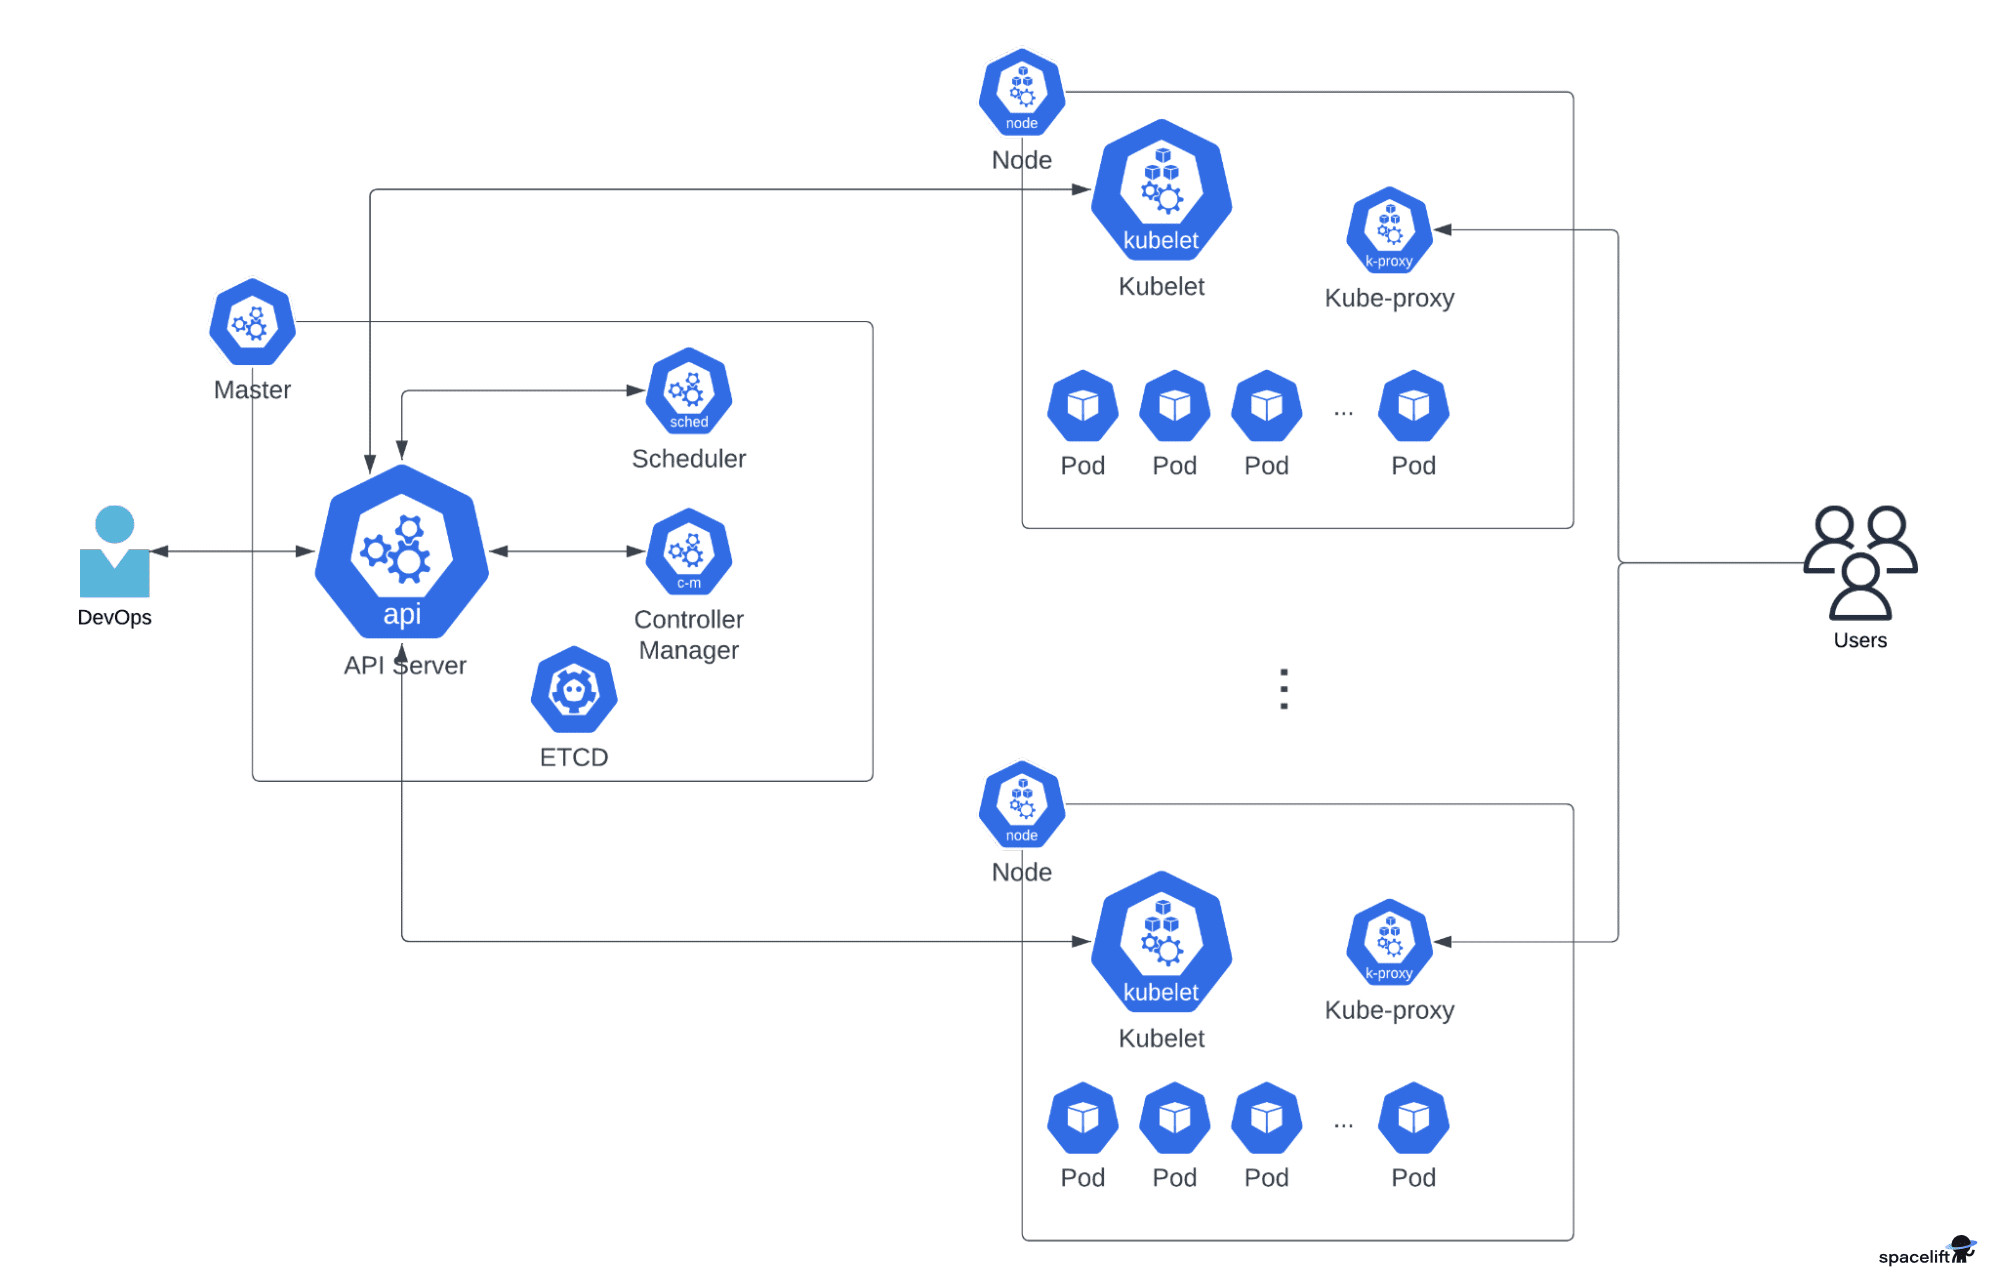
\includegraphics[scale = 0.2]{images/phat/kubernetes_architecture.jpg}
    \vspace*{7mm}
    \caption{Kubernetes Architecture }
    \end{center}
    \label{}
\end{figure}
\indent Kiến trúc của Kubernetes bao gồm:
\begin{itemize}
    \item Master Node: Quản lý, điều phối và giám sát toàn bộ hệ thống Kubernetes.
    \item Worker Node: Chứa các container và chịu trách nhiệm thực hiện các tác vụ đồng bộ từ Master Node.
    \item Pod: Nhóm các container chạy cùng nhau trên cùng một Worker Node, chia sẻ tài nguyên và mạng.
    \item Service: Một tập hợp các Pod có thể truy cập thành một đầu nối duy nhất từ bên ngoài.
    \item Volume: Cung cấp quản lý lưu trữ cho các container trong Pod.
\end{itemize}
\subsubsection{Cách thiết lập Kubernetes cho ứng dụng}
\begin{itemize}
    \item Định nghĩa và triển khai mô tả ứng dụng: Sử dụng các tệp cấu hình (ví dụ: YAML) để định nghĩa ứng dụng, bao gồm Pod, Service và các tài nguyên khác.
    \item Triển khai và quản lý: Gửi yêu cầu triển khai tới Master Node, sau đó Kubernetes sẽ triển khai các Pod và Service, quản lý vòng đời và giám sát.
    \item Tự động mở rộng và cân bằng tải: Kubernetes tự động mở rộng hoặc thu hẹp quy mô của các Pod để đáp ứng tải công việc và cân bằng tải giữa các Worker Node.
\end{itemize}
\subsubsection{Ưu điểm}
\begin{itemize}
    \item Tự động hóa và quản lý quy mô: Kubernetes cho phép tự động mở rộng và thu hẹp quy mô các thành phần ứng dụng, như các microservice và cụm máy chủ. Điều này giúp tối ưu hóa hiệu suất và đáp ứng đối với lưu lượng truy cập thay đổi.

    \item Đảm bảo sẵn lòng và tin cậy: Kubernetes có khả năng phục hồi lỗi tự động và chuyển đổi dịch vụ giữa các phiên bản trên các nút khác nhau. Điều này giúp đảm bảo rằng ứng dụng luôn sẵn sàng và hoạt động một cách tin cậy.

    \item Quản lý tài nguyên hiệu quả: Kubernetes cung cấp các công cụ quản lý tài nguyên để phân bổ và giám sát tài nguyên phù hợp, bao gồm bộ nhớ, CPU, lưu trữ và mạng. Điều này giúp tối ưu hóa sử dụng tài nguyên và tăng hiệu suất hệ thống.

\end{itemize}
\subsubsection{Nhược điểm}
\begin{itemize}
    \item Đòi hỏi kiến thức phức tạp: Kubernetes có độ dốc học và quản lý phức tạp, đòi hỏi kiến thức về hạ tầng và kỹ năng quản lý container.
    \item Tài nguyên tốn kém: Kubernetes yêu cầu sự sẵn có của một cụm máy chủ và tài nguyên đáng kể để triển khai và vận hành.
\end{itemize}
\subsection{Redis Cache}
\subsubsection{Khái niệm}
\indent Redis Cache là một cơ sở dữ liệu key-value (khóa-giá trị) phân tán, được sử dụng để lưu trữ dữ liệu tạm thời trong bộ nhớ. \footnote{https://kdata.vn/cam-nang/redis-la-gi-hieu-ro-ve-he-thong-co-so-du-lieu-trong-bo-nho}
\subsubsection{Ưu điểm}
\begin{itemize}
    \item Tốc độ và hiệu suất cao: Redis Cache lưu trữ dữ liệu trong bộ nhớ và cho phép truy cập cực kỳ nhanh chóng, đáp ứng yêu cầu với hiệu suất cao.
    \item Đa dạng tính năng: Redis cung cấp nhiều tính năng như caching, xử lý hàng đợi, pub/sub messaging và phân tích dữ liệu, giúp tối ưu hóa các tác vụ dựa trên dữ liệu.
\end{itemize}
\subsubsection{Nhược điểm}
\begin{itemize}
    \item Giới hạn bộ nhớ: Redis Cache yêu cầu bộ nhớ đủ lớn để lưu trữ dữ liệu. Nếu dữ liệu vượt quá dung lượng bộ nhớ, có thể gặp sự cố và ảnh hưởng đến hiệu suất.
    \item Khả năng mất dữ liệu: Redis Cache mặc định không cung cấp cơ chế đồng bộ hoá dữ liệu, điều này đồng nghĩa rằng có thể mất dữ liệu khi xảy ra sự cố.
\end{itemize}
\subsection{PostgreSQL}
\subsubsection{Khái niệm}
\indent PostgreSQL (viết tắt là Postgres) là một hệ quản trị cơ sở dữ liệu quan hệ mã nguồn mở, được đánh giá là ổn định, mạnh mẽ và có tính mở rộng.
\subsubsection{Ưu điểm}
\begin{itemize}
    \item Độ tin cậy cao: PostgreSQL được thiết kế để đảm bảo tính toàn vẹn và độ tin cậy của dữ liệu, bao gồm các tính năng như ACID và khả năng khôi phục dữ liệu.
    \item Tính mở rộng và phân vùng: PostgreSQL hỗ trợ phân vùng dữ liệu và khả năng mở rộng sẵn sàng, cho phép mở rộng cơ sở dữ liệu để xử lý lượng dữ liệu lớn và tải cao.
    \item Đa dạng tính năng: PostgreSQL cung cấp nhiều tính năng tiên tiến bao gồm trình tự, trigger, tìm kiếm văn bản và hình ảnh, và hỗ trợ các loại dữ liệu phong phú.
\end{itemize}
\subsubsection{Nhược điểm}
\begin{itemize}
    \item Có thể cảm thấy phức tạp đối với các dự án nhỏ.
\end{itemize}
\subsection{EKS}
\subsubsection{Khái niệm}
\indent EKS (Elastic Kubernetes Service) là một dịch vụ quản lý Kubernetes do Amazon Web Services (AWS) cung cấp.
\subsubsection{Ưu điểm}
\begin{itemize}
    \item Dễ dàng triển khai, quản lý và mở rộng các ứng dụng chạy trên Kubernetes.
    \item Tích hợp tốt với dịch vụ AWS khác.
    \item Hỗ trợ cho môi trường đám mây tiêu chuẩn và quy mô lớn.
\end{itemize}
\subsubsection{Nhược điểm}
\begin{itemize}
    \item Phí sử dụng có thể cao, đặc biệt trong trường hợp triển khai lớn.
    \item Đòi hỏi kiến thức về quản lý và triển khai hệ thống phức tạp hơn so với các giải pháp khác.
\end{itemize}
\subsection{AKS}
\subsubsection{Khái niệm}
\indent AKS (Azure Kubernetes Service) là một dịch vụ quản lý Kubernetes.

\subsubsection{Ưu điểm}
\begin{itemize}
    \item Dễ dàng triển khai, quản lý và mở rộng các ứng dụng chạy trên Kubernetes.
    \item Tích hợp tốt với dịch vụ Azure và công cụ phát triển của Microsoft.
    \item Cung cấp tính năng bảo mật và giám sát mạnh mẽ.
\end{itemize}
\subsubsection{Nhược điểm}
\begin{itemize}
    \item Phí sử dụng có thể cao, đặc biệt trong trường hợp triển khai lớn.
    \item Yêu cầu sử dụng môi trường và công cụ phát triển Azure.
\end{itemize}
\subsection{RabbitMQ}
\subsubsection{Khái niệm}
\indent RabbitMQ là một hệ thống message broker mã nguồn mở, dựa trên giao thức AMQP (Advanced Message Queuing Protocol).\\
Hình ảnh được thảm khảo từ bài viết "An introduction to RabbitMQ – What is RabbitMQ?"\footnote{https://www.erlang-solutions.com/blog/an-introduction-to-rabbitmq-what-is-rabbitmq/} 
\begin{figure}[H]

    \begin{center}
    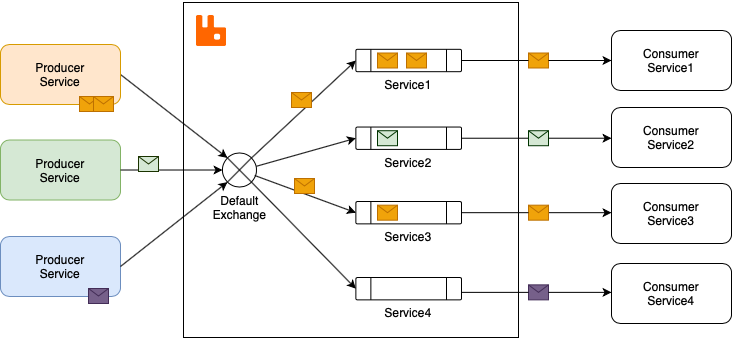
\includegraphics[scale = 0.5]{images/phat/rabbitMQ.png}
    \vspace*{7mm}
    \caption{RabbitMQ Architecture}
    \end{center}
    \label{}
\end{figure}
\subsubsection{Kiến trúc của RabbitMQ}
\begin{itemize}
    \item Producer:

Là thành phần tạo ra và gửi các thông điệp (message).
Message được gửi đến một exchange.
    \item Exchange:

Nhận thông điệp từ nhà sản xuất và định tuyến chúng đến hàng đợi (queue) thích hợp.
Có các loại định tuyến khác nhau như direct, topic, fanout, và headers, cho phép định tuyến dựa trên các tiêu chí khác nhau.
    \item Queue (Hàng đợi):

Là nơi lưu trữ các thông điệp đến từ sàn giao dịch cho đến khi chúng được xử lý bởi một tiêu thụ (consumer).
Các hàng đợi có thể được chia sẻ giữa nhiều tiêu thụ hoặc có thể chỉ được sử dụng bởi một tiêu thụ cụ thể.
    \item Binding (Ràng buộc):

Liên kết giữa một exchange và một queue, xác định cách thông điệp nên được định tuyến từ exchange đến queue.
Ràng buộc này được thiết lập thông qua các quy tắc định tuyến (routing key).
    \item Consumer:

Là thành phần đọc và xử lý các thông điệp từ hàng đợi.
Có thể có nhiều tiêu thụ cùng một lúc đọc từ cùng một hàng đợi.
    \item Virtual Host:

Là một không gian làm việc ảo trong RabbitMQ, giúp tách biệt và cô lập các ứng dụng và người dùng khác nhau.
Mỗi Virtual Host có thể có các exchange, queue, và quyền riêng biệt.
    \item Broker:

Là nền tảng hoạt động của RabbitMQ.
Nhận thông điệp từ nhà sản xuất, định tuyến chúng đến hàng đợi thông qua sàn giao dịch và chuyển giao chúng đến các tiêu thụ.
    \item Connection:

Là một kết nối mạng giữa ứng dụng và RabbitMQ Broker.
Mỗi ứng dụng có thể có nhiều kết nối.
\end{itemize}

\subsubsection{Ưu điểm}
\begin{itemize}
    \item Hỗ trợ đa ngôn ngữ và dễ dàng tích hợp với các ứng dụng phổ biến.
    \item Cung cấp tính năng đám mây phân tán, đảm bảo bất đồng bộ và xử lý hàng đợi.
    \item Tích hợp tốt với các công nghệ và framework khác như Spring, .NET, Node.js, etc.
\end{itemize}
\subsubsection{Nhược điểm}
\begin{itemize}
    \item Cấu hình phức tạp và yêu cầu kiến thức về hệ thống phân tán.
    \item Hiệu suất có thể bị ảnh hưởng đối với tải công việc rất cao.
\end{itemize}

\section{Định nghĩa các yêu cầu mục tiêu của đồ án}
\noindent Đề tài xây dựng nhằm phân tích và giải quyết bài toán xoay quanh 2 từ khóa \textbf{scalability} và \textbf{availability}. Do đó, ta cần đi vào tìm hiểu định nghĩa của 2 từ khóa này:
% \\[0.5cm]

\subsection{Availability - Tính sẵn sàng}
\noindent Theo định nghĩa của Microsoft\footnote{Website: https://learn.microsoft.com/en-us/training/modules/describe-benefits-use-cloud-services/2-high-availability-scalability-cloud}, “Khi bạn deploy một ứng dụng, dịch vụ, hay bất kỳ tài nguyên IT nào, việc những tài nguyên đó sẵn sàng khi bạn cần là điều quan trọng. High availability tập trung vào việc đảm bảo tối đa tính sẵn sàng của hệ thống, bất kể sự gián đoạn hay sự kiện nào có thể xảy ra.” \\[0.5cm]
\noindent Khi xây dựng giải pháp của mình, ta sẽ cần tính đến các đảm bảo về tính khả dụng của dịch vụ. Azure là môi trường đám mây có tính sẵn sàng cao với sự đảm bảo về thời gian hoạt động tùy thuộc vào dịch vụ. Những đảm bảo này là một phần của thỏa thuận cấp độ dịch vụ (SLA).
\noindent Công thức tính availability của hệ thống là:\\
\begin{equation}
    Availability = \frac{Operational Time}{Total Time}\\
\end{equation}
\noindent Trong đó:
\begin{itemize}
    \item OperationalTime là thời gian hệ thống hoạt động và sẵn sàng.
    \item TotalTime là tổng thời gian trong khoảng thời gian nhất định.
\end{itemize}
\subsection{Scalability - Tính mở rộng}
\noindent Theo định nghĩa của Microsoft\footnote{Như trên}, “Khả năng mở rộng (scalability) đề cập đến khả năng điều chỉnh các tài nguyên để đáp ứng nhu cầu. Nếu bạn đột nhiên gặp phải lưu lượng truy cập cao và hệ thống của bạn bị quá tải thì khả năng mở rộng quy mô có nghĩa là bạn có thể bổ sung thêm tài nguyên để xử lý tốt hơn lượng tải đang gia tăng.” \\[0.5cm]
\noindent Lợi ích khác của tính mở rộng là bạn không phải trả quá nhiều tiền cho các dịch vụ. Vì đám mây là mô hình dựa trên mức tiêu dùng nên bạn chỉ trả tiền cho những gì bạn sử dụng. Nếu nhu cầu giảm, bạn có thể giảm tài nguyên và từ đó giảm chi phí. \\[0.5cm]
\noindent Scalability thường có hai loại: dọc và ngang. Mỏ rộng theo chiều dọc tập trung vào việc tăng hoặc giảm khả năng của tài nguyên. Mở rộng theo chiều ngang là thêm hoặc bớt số lượng tài nguyên.

\section{Định nghĩa các kiểu kiến trúc hệ thống}
\noindent Nội dung dưới đây tham khảo từ module \textit{Decompose a monolithic application into a microservices architecture} của Microsoft Learn.\footnote{Website: https://learn.microsoft.com/en-us/training/modules/microservices-architecture/}
\subsection{Kiến trúc monolith}
\subsubsection{Định nghĩa}
\noindent Kiến trúc monolith là kiến trúc trong đó tất cả các thành phần của một ứng dụng được đặt trong một đơn vị duy nhất. Đơn vị này thường bị hạn chế trong một phiên bản thời gian chạy duy nhất của ứng dụng. Các ứng dụng truyền thống thường bao gồm giao diện web, lớp dịch vụ và lớp dữ liệu. Trong kiến trúc monolith, các lớp này được kết hợp trên một phiên bản của ứng dụng.
\subsubsection{Lý do sử dụng}
Kiến trúc monolith thường là giải pháp phù hợp cho các ứng dụng nhỏ, nhưng chúng có thể trở nên khó sử dụng khi ứng dụng phát triển. Ban đầu, một ứng dụng nhỏ có thể nhanh chóng trở thành một hệ thống phức tạp, khó mở rộng quy mô, khó triển khai và khó đổi mới.
\subsubsection{Thách thức}
Tất cả các dịch vụ được chứa trong một đơn vị duy nhất. Sự sắp xếp này mang lại những thách thức khi hoạt động kinh doanh của họ và tải hệ thống tiếp theo phát triển. Một số thách thức này là:
\begin{itemize}
    \item Khó mở rộng quy mô dịch vụ một cách độc lập.
    \item Phức tạp để phát triển và quản lý việc triển khai khi cơ sở mã phát triển, điều này làm chậm quá trình phát hành và triển khai tính năng mới.
    \item Kiến trúc được gắn với một ngăn xếp công nghệ duy nhất, điều này hạn chế sự đổi mới trong các nền tảng và SDK mới.
    \item Cập nhật lược đồ dữ liệu có thể ngày càng khó khăn.
\end{itemize}
Những thách thức này có thể được giải quyết bằng cách xem xét các kiến trúc thay thế, chẳng hạn như kiến trúc microservices.

\subsection{Kiến trúc microservices}
\subsubsection{Định nghĩa}
Kiến trúc microservice bao gồm các dịch vụ nhỏ, độc lập và được liên kết lỏng lẻo. Mỗi dịch vụ có thể được triển khai và mở rộng quy mô một cách độc lập.\\[0.5cm]
Một microservice đủ nhỏ để một nhóm nhỏ các nhà phát triển có thể viết và duy trì nó. Vì các dịch vụ có thể được triển khai độc lập nên một nhóm có thể cập nhật dịch vụ hiện có mà không cần xây dựng lại và triển khai lại toàn bộ ứng dụng.\\[0.5cm]
Mỗi dịch vụ thường chịu trách nhiệm về dữ liệu riêng của mình. Cấu trúc dữ liệu của nó được tách biệt nên việc nâng cấp hoặc thay đổi lược đồ không phụ thuộc vào các dịch vụ khác. Các yêu cầu về dữ liệu thường được xử lý thông qua API và cung cấp mô hình truy cập nhất quán và được xác định rõ ràng. Chi tiết triển khai nội bộ được ẩn khỏi người tiêu dùng dịch vụ.\\[0.5cm]
Vì mỗi dịch vụ đều độc lập nên chúng có thể sử dụng các nhóm công nghệ, khung và SDK khác nhau. Người ta thường thấy các dịch vụ dựa vào các lệnh gọi REST để liên lạc giữa các dịch vụ bằng cách sử dụng các API được xác định rõ ràng thay vì các lệnh gọi thủ tục từ xa (RPC) hoặc các phương thức liên lạc tùy chỉnh khác.\\[0.5cm]
Kiến trúc vi dịch vụ không phụ thuộc vào công nghệ, nhưng bạn thường thấy các bộ chứa hoặc công nghệ serverless được sử dụng để triển khai chúng. Triển khai liên tục và tích hợp liên tục (CI/CD) thường được sử dụng để tăng tốc độ và chất lượng của các hoạt động phát triển.
\subsubsection{Lý do sử dụng}
Có một số lợi ích chính đối với kiến trúc microservices:
\begin{itemize}
    \item Nhanh nhẹn
    \item Mã nhỏ, nhóm nhỏ
    \item Sự kết hợp của công nghệ
    \item khả năng phục hồi
    \item Khả năng mở rộng (Scalability)
    \item Cách ly dữ liệu
\end{itemize}
\subsubsection{Những thách thức}
Có rất nhiều lợi ích đối với kiến trúc microservices, nhưng đó không phải là tất cả. Kiến trúc microservice có những thách thức riêng:
\begin{itemize}
    \item Độ phức tạp
    \item Phát triển và thử nghiệm
    \item Thiếu quản trị
    \item Tắc nghẽn mạng và độ trễ
    \item Toàn vẹn dữ liệu
    \item Sự quản lý
    \item Phiên bản
    \item Bộ kỹ năng    
\end{itemize}
\textbf{Khi nào nên chọn kiến trúc microservices?}\\[0.5cm]
Dựa vào những thông tin trên, kiến trúc microservices sẽ phù hợp trong những tình huống sau
\begin{itemize}
    \item Các ứng dụng lớn đòi hỏi tốc độ phát hành cao.
    \item Các ứng dụng phức tạp cần có khả năng mở rộng cao.
    \item Ứng dụng có miền phong phú hoặc nhiều miền phụ.
    \item Một tổ chức bao gồm các nhóm phát triển nhỏ.    
\end{itemize}

\newpage
\section{Case study}
\subsection{Ứng dụng kiến trúc microservice với Azure Kubernetes Service}
\noindent Tham khảo từ bài viết "Microservices architecture on Azure Kubernetes Service" trên Microsoft Learn.\footnote{Nguồn tham khảo: https://learn.microsoft.com/en-us/azure/architecture/reference-architectures/containers/aks-microservices/aks-microservices}
\begin{figure}[H]
    \begin{center}
    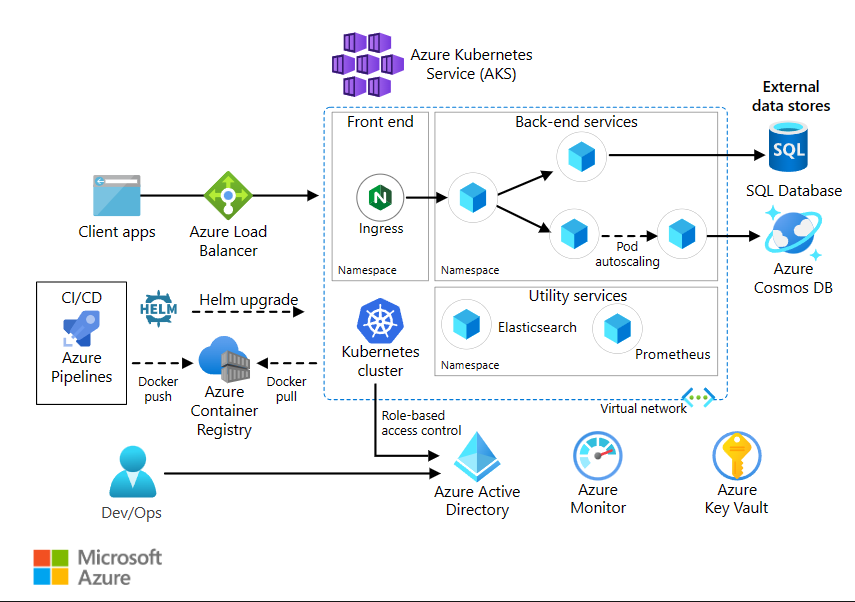
\includegraphics[scale=0.8]{images/hieu/chap-2/aks-architecture.png}
    \vspace*{5mm}
    \caption{AKS Architecture}
    \end{center}
\end{figure}
\subsubsection{Các thành phần của kiến trúc}
\begin{itemize}
    \item \textbf{Azure Kubernetes Service (AKS)}: Là một dịch vụ quản lý Kubernetes do Microsoft cung cấp. Azure quản lý dịch vụ API Kubernetes và bạn chỉ cần quản lý các nút tác nhân (agent node).
    \item \textbf{Virtual Network}: Theo mặc định, AKS tạo một mạng ảo trong đó các nút tác nhân được kết nối. Trước tiên, bạn có thể tạo mạng ảo cho các tình huống nâng cao hơn, cho phép bạn kiểm soát những thứ như cấu hình mạng con.
    \item \textbf{Ingress}: Ingress hiển thị các tuyến HTTPs tới các dịch vụ bên trong cluster.
    \item \textbf{Azure Load Balancer}: Sau khi tạo AKS cluster, cluster đã sẵn sàng sử dụng bộ cân bằng tải. Khi dịch vụ NGINX được triển khai, bộ cân bằng tải sẽ được cấu hình bằng một IP công cộng mới phía trước bộ điều khiển xâm nhập (ingress controller). Bằng cách này, bộ cân bằng tải định tuyến lưu lượng truy cập internet đến ingress.
    \item \textbf{Exteral Data Store}: Các microservice thường không có trạng thái (stateless) và trạng thái ghi vào các kho dữ liệu bên ngoài, chẳng hạn như Cơ sở dữ liệu Azure SQL hoặc Azure Cosmos DB.
    \item \textbf{Microsoft ID Entra}: AKS sử dụng Microsoft Entra ID để tạo và quản lý các tài nguyên Azure khác như bộ cân bằng tải Azure. Microsoft Entra ID cũng được khuyến nghị để xác thực người dùng trong các ứng dụng khách.
    \item \textbf{Azure Container Registry}: Azure Container Registry là một kho lưu trữ riêng tư cho các hình ảnh Docker. Nó được sử dụng để lưu trữ các hình ảnh Docker được sử dụng để triển khai các dịch vụ trong AKS cluster.
    \item \textbf{Azure Pipeline}: Azure Pipeline là một dịch vụ liên tục tích hợp và triển khai (CI/CD) được sử dụng để triển khai các dịch vụ trong AKS cluster.. Azure Pipelines là một phần của Dịch vụ Azure DevOps và chạy các bản dựng, thử nghiệm và triển khai tự động.
    \item \textbf{Helm}: Helm là một công cụ quản lý gói cho Kubernetes. Nó cho phép bạn định nghĩa, cài đặt và cập nhật các ứng dụng Kubernetes. Helm Charts là các gói Helm. Helm Charts được sử dụng để triển khai các ứng dụng trong AKS cluster.
    \item \textbf{Azure Monitor}: Azure Monitor là một dịch vụ giám sát đám mây. Nó cho phép bạn thu thập và phân tích dữ liệu từ nhiều nguồn khác nhau, bao gồm các dịch vụ Azure và các ứng dụng trên nhiều nền tảng. Azure Monitor được sử dụng để giám sát các dịch vụ trong AKS cluster.
\end{itemize}
\subsubsection{Một số cân nhắc}
\begin{itemize}
    \item \textbf{Design}: Kiến trúc tham chiếu này tập trung vào kiến trúc microservice, mặc dù nhiều phương pháp được đề xuất áp dụng cho các khối lượng công việc khác chạy trên AKS.
    \item \textbf{Microservice}: Microservice là một đơn vị mã có thể triển khai độc lập. Các microservice thường giao tiếp thông qua các API được xác định rõ ràng . Dịch vụ phải luôn có thể truy cập được ngay cả khi pod di chuyển xung quanh. Đối tượng Dịch vụ Kubernetes là một cách tự nhiên để mô hình hóa các dịch vụ vi mô trong Kubernetes.
    \item \textbf{API Gateway}: API gateway nằm giữa các máy khách bên ngoài và microservice. Nó hoạt động như một proxy ngược, định tuyến các yêu cầu từ máy khách đến microservice.
    \item \textbf{Data storage}: Trong kiến trúc microservice, các dịch vụ không nên chia sẻ giải pháp lưu trữ dữ liệu. Mỗi dịch vụ nên quản lý tập dữ liệu riêng của mình để tránh sự phụ thuộc ẩn giữa các dịch vụ.
Tránh lưu trữ dữ liệu liên tục trong bộ lưu trữ cluster cục bộ vì điều đó liên kết dữ liệu với node. Thay vào đó, hãy sử dụng dịch vụ bên ngoài như Cơ sở dữ liệu Azure SQL hoặc Azure Cosmos DB. Nếu bạn cần lưu trữ dữ liệu tạm thời, hãy sử dụng Redis Cache.
    \item \textbf{Namespace}: Namespace tổ chức các dịch vụ trong cluster, ngăn ngừa xung đột tên, áp dụng ràng buộc tài nguyên và chính sách bảo mật ở cấp độ namespace, và tổ chức microservice thành các ngữ cảnh được giới hạn thông qua việc tạo namespace cho từng ngữ cảnh. Đồng thời, việc đặt các dịch vụ tiện ích như Elasticsearch, Prometheus hoặc Tiller vào các namespace riêng biệt cũng được khuyến khích.
    \item \textbf{Health Probes}: Health probes là các yêu cầu HTTP được gửi đến các dịch vụ để xác định trạng thái của chúng. Nếu một dịch vụ không phản hồi, Kubernetes sẽ xóa pod và tạo lại nó. Điều này đảm bảo rằng các dịch vụ luôn sẵn sàng để phục vụ yêu cầu.
    \\[0.5cm]
    Kubernetes xác định hai loại thăm dò sức khỏe mà pod có thể hiển thị:
        \begin{itemize}
            \item Thăm dò sẵn sàng: Thăm dò sẵn sàng xác định khi nào pod đã sẵn sàng để phục vụ yêu cầu.  
            \item Thăm dò sự sống: Thăm dò sự sống xác định khi nào pod cần được khởi động lại. Nếu thăm dò sự sống thất bại, pod sẽ bị xóa và tạo lại.
        \end{itemize}
    Một số cân nhắc khi thiết kế health probes:
        \begin{itemize}
            \item Nếu mã của bạn có thời gian khởi động dài, có nguy cơ do trình thăm dò mức độ hoạt động sẽ báo cáo lỗi trước khi quá trình khởi động hoàn tất. Để giải quyết vấn đề này, hãy sử dụng cài đặt initialDelaySeconds để trì hoãn việc khởi động đầu dò.
            \item Việc thăm dò độ sống sẽ không giúp ích gì trừ khi việc khởi động lại pod có khả năng khôi phục nó về trạng thái khỏe mạnh. Bạn có thể sử dụng công cụ thăm dò mức độ hoạt động để giảm thiểu tình trạng rò rỉ bộ nhớ hoặc bế tắc không mong muốn, nhưng việc khởi động lại pod sẽ lại bị lỗi ngay lập tức sẽ chẳng ích gì.
            \item Đôi khi các thăm dò sẵn sàng được sử dụng để kiểm tra các dịch vụ phụ thuộc. 
            Ví dụ: nếu một pod phụ thuộc vào cơ sở dữ liệu thì đầu dò có thể kiểm tra kết nối cơ sở dữ liệu. 
            Tuy nhiên, cách tiếp cận này có thể tạo ra những vấn đề không mong muốn. 
            Một dịch vụ bên ngoài có thể tạm thời không khả dụng vì một số lý do. 
            Điều đó sẽ khiến cho việc thăm dò mức độ sẵn sàng không thành công đối với tất cả các pod trong dịch vụ của bạn, khiến tất cả các pod đó bị xóa khỏi cân bằng tải và do đó tạo ra lỗi xếp tầng ở thượng nguồn. 
            Cách tiếp cận tốt hơn là triển khai xử lý thử lại trong dịch vụ của bạn để dịch vụ của bạn có thể khôi phục chính xác sau các lỗi nhất thời.
        \end{itemize}
    \item \textbf{Resource constrain}: Tranh chấp tài nguyên có thể ảnh hưởng đến tính sẵn có của dịch vụ. Xác định các giới hạn tài nguyên cho các container để một container không thể áp đảo các tài nguyên của cluster (bộ nhớ và CPU).
    Sử dụng hạn ngạch tài nguyên để giới hạn tài nguyên được phép cho một namespace. 
    \item \textbf{Service object - SO}: Đối tượng dịch vụ Kubernetes cung cấp một tập hợp các khả năng phù hợp với yêu cầu của microservice về khả năng khám phá dịch vụ:
        \begin{itemize}
            \item Địa chị IP: SO cung cấp một địa chỉ IP nội bộ tĩnh cho một pod (ReplicaSet) để các dịch vụ có thể truy cập tại địa chỉ này.
            \item Cân bằng tải (Load Balancer): Lưu lượng gửi đến địa chỉ IP của dịch vụ được cân bằng tải cho cácp pod.
            \item Khám phá dịch vụ (Service Recovery): SO cung cấp một tên miền DNS cho một dịch vụ, cổng API có thể gọi dịch vụ bằng tên miền này này. Các mục DNS được sắp xếp theo namespace.
        \end{itemize}
        \begin{figure}[H]
            \centering
            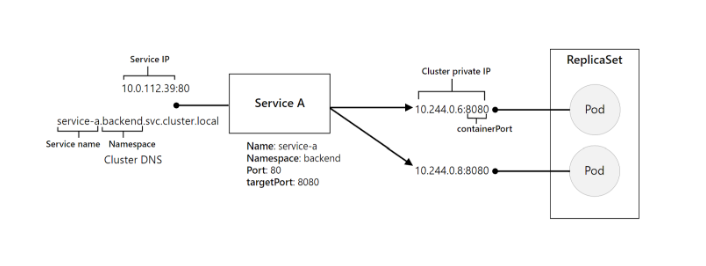
\includegraphics[scale=1]{images/hieu/chap-2/service-object-diagram.png}
            \vspace*{5mm}
            \caption{Sơ đồ mối quan hệ giữa các đối tượng dịch vụ và pod}
        \end{figure}
    \item \textbf{Ingress}: Bộ điều khiển ingress (Ingress Controller) và ingress có thể phối hợp hoạt động để cung cấp các tính năng sau:
        \begin{itemize}
            \item Định tuyến các yêu cầu của khách hàng, định tuyến này cung cấp một điểm cuối duy nhất cho khách hàng và tách khách hàng khỏi các dịch vụ.
            \item Tổng hợp nhiều yêu cầu thành một yêu cầu duy nhất.
            \item Giảm tải chức năng như chấm dứt SSL, xác thực, hạn chế IP hoặc giới hạn tốc độ máy khách. 
        \end{itemize}
    \item \textbf{Mã hoá TLS/SSL}: Mã hoá TLS/SSL là một phương pháp mã hoá dữ liệu để bảo mật các kết nối giữa các máy khách và máy chủ.
\end{itemize}
\subsubsection{Security}
\begin{itemize}
    \item \textbf{Role-based Access Control}
    \newline
    Kubernetes và Azure đều có cơ chế kiểm soát truy cập dựa trên vai trò (RBAC):
    \begin{itemize}
        \item Azure RBAC kiểm soát quyền truy cập vào tài nguyên trong Azure, bao gồm khả năng tạo tài nguyên mới. Quyền có thể được chỉ định cho người dùng.
        \item Kubernetes RPAC kiểm soát các quyền đối với API Kubernetes. Để gán quyền Kubernetes cho người dùng, tạo vai trò và ràng buộc vai trò với người dùng.
    \end{itemize}
    AKS tích hợp hai chơ chế RBAC này, khi tạo một cụm AKS, bạn có thể đặt cấu hình cụm đó để sử dụng Microsoft Entra ID để xác thực người dùng. Người dùng Microsoft Entra ID cần được quản trị viên cụm tạo RoleBindings để cấp quyền truy cập cho người dùng hoặc nhóm người dùng.
    \item \textbf{Secrets management and application credentials}
    \newline
    Các ứng dụng và dịch vụ thường cần thông tin xác thực cho phép chúng kết nối với các dịch vụ bên ngoài như Bộ lưu trữ Azure hoặc Cơ sở dữ liệu SQL. Thách thức là giữ những thông tin xác thực này an toàn và không rò rỉ chúng.
    Dưới đây là một số tuỳ chọn để lưu trữ bí mật một cách an toàn:
        \begin{itemize}
            \item Azure Key Vault: Azure Key Vault là một dịch vụ quản lý khóa, bí mật và chứng chỉ. Nó cung cấp một nơi để lưu trữ các bí mật và khóa truy cập vào các dịch vụ bên ngoài. Các ứng dụng có thể truy cập Key Vault để lấy thông tin xác thực.
            \item Kubernetes Secrets: Kubernetes Secrets là một đối tượng Kubernetes được sử dụng để lưu trữ các bí mật. Các bí mật được lưu trữ dưới dạng cặp khóa-giá trị và có thể được sử dụng bởi các pod trong cụm.
            \item HashiCorp Vault: HashiCorp Vault là một dịch vụ quản lý khóa, bí mật và chứng chỉ mã nguồn mở. Nó cung cấp một nơi để lưu trữ các bí mật và khóa truy cập vào các dịch vụ bên ngoài. Các ứng dụng có thể truy cập Vault để lấy thông tin xác thực.
        \end{itemize}
    Việc sử dụng HashiCorp Vault hoặc Azure Key Vault là một giải pháp tốt hơn so với Kubernetes Secrets có thể mang lại mốt số lợi ích:
        \begin{itemize}
            \item Kiểm soát tập trung các bí mật
            \item Đảm bảo ràng tất cả các bí mật được mã hoá ở phần còn lại.
            \item Quản lý khoá tập trung.
            \item Kiểm soát truy cập bị mật.
            \item Kiểm toán.
        \end{itemize}
    \item \textbf{Container và Orchestrator security} đây là những phương pháp được khuyến nghị để bảo vệ pods và container của bạn:

        \begin{itemize}
            \item Giám sát mối đe doạ (thread monitoring) bằng cách sử dụng Microsoft Defender cho Containers.
            \item Giám sát lỗ hổng (Vulnerabilities monitoring) bằng cách sử dụng Microsoft Defender dành cho đám mây hoặc giải pháp bên thứ ba có sẵn thông qua Azure Marketplace.
            \item Tự động vá hình ảnh bằng tác vụ ACR, một tính năng của Azure Register. 
            \item Lưu trữ image trong Azure Container Registry, một private registry đáng tin cậy. Sử dụng webhook xác thực tiếp nhận trong Kubernetes để đảm bảo rằng các nhóm chỉ có thể lấy hình ảnh từ cơ quan đăng ký đáng tin cậy.
        \end{itemize}
      
\end{itemize}
\newpage
\subsection {Ứng dụng AKS cho kiến trúc microservice nâng cao}
\noindent Tham khảo từ bài viết "Advanced Azure Kubernetes Service (AKS) microservices architecture" từ Microsoft Learn.\footnote{Nguồn tham khảo: https://learn.microsoft.com/en-us/azure/architecture/reference-architectures/containers/aks-microservices/aks-microservices-advanced}
\begin{figure}[H]
    \centering
    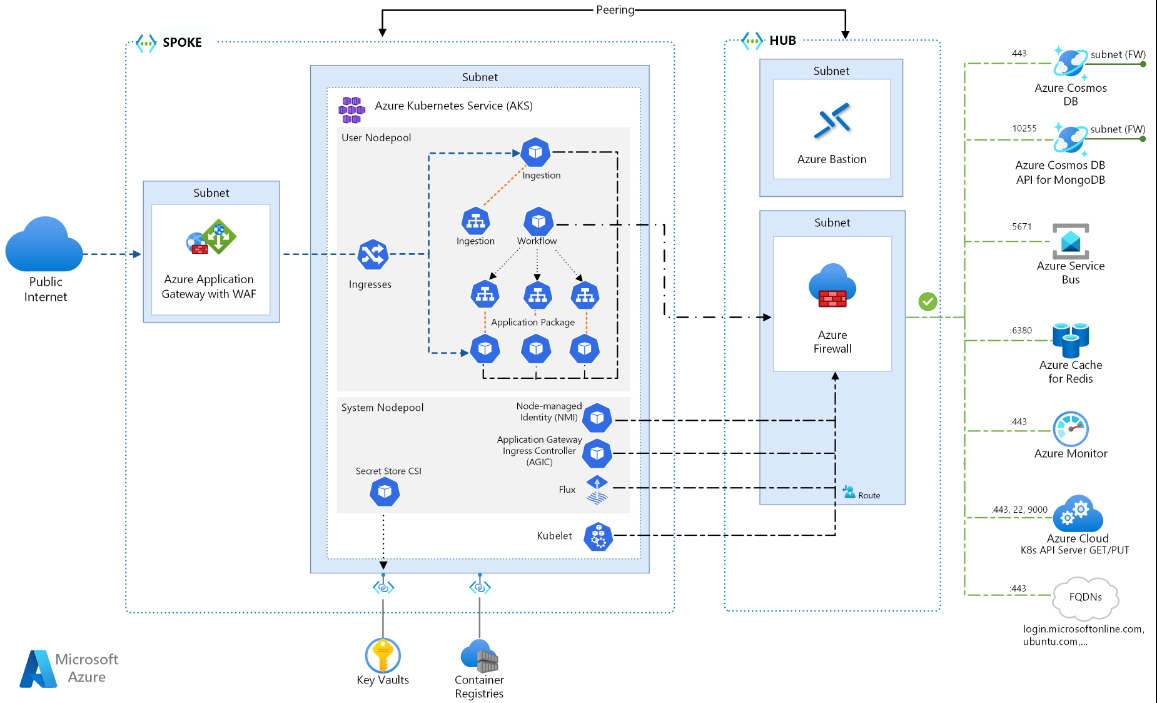
\includegraphics[scale=0.6]{images/hieu/chap-2/aks-architecture-advance.png}
    \caption{AKS Architecture Advance}
\end{figure}
\subsubsection{Workflow}
Luồng yêu cầu này triển khai các design pattern trên cloud Publisher-Subscriber, Competing Consumers, và Gateway Routing. Luồng tin nhắn diễn ra như sau:
    \begin{itemize}
        \item Một yêu cầu HTTPS được gửi để lên lịch nhận hàng bằng máy bay không người lái. Các yêu cầu chuyển qua Cổng ứng dụng Azure vào ứng dụng web nhập, ứng dụng này chạy dưới dạng vi dịch vụ trong cụm trong AKS.
        \item Ứng dụng web truyền dẫn sẽ tạo một thông báo và gửi nó đến hàng đợi thông báo Service Bus.
        \item Hệ thống phụ trợ chỉ định một máy bay không người lái và thông báo cho người dùng. Quy trình làm việc:
            \begin{itemize}
                \item Sử dụng thông tin tin nhắn từ hàng đợi tin nhắn Service Bus.
                \item Gửi yêu cầu HTTPS tới vi dịch vụ Phân phối để chuyển dữ liệu tới Bộ nhớ đệm Azure để lưu trữ dữ liệu ngoài của Redis.
                \item Gửi yêu cầu HTTPS tới microservice Drone Scheduler. 
                \item Gửi yêu cầu HTTPS tới vi dịch vụ Package, chuyển dữ liệu tới bộ lưu trữ dữ liệu bên ngoài MongoDB.
            \end{itemize} 
        \item Yêu cầu HTTPS GET được sử dụng để trả về trạng thái gửi. Yêu cầu này đi qua Cổng ứng dụng vào vi dịch vụ phân phối (Delivery Microservice).
        \item Vi dịch vụ phân phối đọc dữ liệu từ Azure Cache cho Redis.     
    \end{itemize}
\subsubsection{Các thành phần của kiến trúc}
Kiến trúc này sử dụng các thành phần Azure sau:
\begin{itemize}
    \item \textbf{Azure Kubernetes Services} là một dịch vụ Azure cung cấp cụm Kubernetes được quản lý. Khi sử dụng AKS, máy chủ API Kubernetes được quản lý bởi Azure. Các nút hoặc nhóm nút Kubernetes có thể truy cập được và được quản lý bởi nhà điều hành cụm.
    Các tính năng AKS sủe dụng trong kiến trúc này bao gồm:
    \begin{itemize}
        \item Tách nhóm node hệ thống và người dùng
        \item ID Microsoft Entra do AKS quản lý để kiểm soát truy cập dựa trên vai trò (RBAC)
        \item ID khối lượng công việc Microsoft Entra
        \item Tiện ích bổ sung chính sách Azure cho AKS
        \item Giao diện mạng vùng chứa Azure (CNI)
        \item Thông tin chi tiết về vùng chứa Azure Monitor
    \end{itemize} 
    \item \textbf{Azure Virtual Network} là môi trường biệt lập và có độ bảo mật cao để chạy các ứng dụng và máy ảo (VM). Kiến trúc tham chiếu này sử dụng cấu trúc liên kết mạng ảo trung tâm ngang hàng. Mạng ảo trung tâm chứa tường lửa Azure và mạng con Azure Bastion. Mạng ảo nan hoa chứa các mạng con nhóm nút người dùng và hệ thống AKS cũng như mạng con cổng ứng dụng Azure.
    \item  \textbf{Azure Private Link} phân bổ các địa chỉ IP riêng tư cụ thể để truy cập Azure Container Register và Key Vault từ Điểm cuối riêng tư trong hệ thống AKS và mạng con nhóm nút người dùng.
    \item \textbf{Azure Application Gateway} với tường lửa ứng dụng web (WAF) hiển thị các tuyến HTTP(S) tới cụm AKS và cân bằng tải lưu lượng truy cập web đến ứng dụng web. Kiến trúc này sử dụng Bộ điều khiển xâm nhập cổng ứng dụng Azure (AGIC) làm bộ điều khiển xâm nhập Kubernetes.
    \item \textbf{Azure Bastion} cung cấp giao thức máy tính từ xa an toàn (RDP) và quyền truy cập shell bảo mật (SSH) vào máy ảo trong mạng ảo bằng cách sử dụng lớp ổ cắm bảo mật (SSL) mà không cần hiển thị máy ảo thông qua địa chỉ IP công cộng.
    \item \textbf{Azure Firewall} là dịch vụ bảo mật mạng bảo vệ tất cả tài nguyên Mạng ảo Azure. Tường lửa chỉ cho phép các dịch vụ được phê duyệt và tên miền đủ điều kiện (FQDN) làm lưu lượng truy cập đầu ra. 
\end{itemize}
\subsubsection{Bộ nhớ ngoài (external storage) và các thành phần khác}
\begin{itemize}
    \item \textbf{Azure Container Register} lưu trữ các hình ảnh vùng chứa riêng tư có thể chạy trong cụm AKS. AKS xác thực với Cơ quan đăng ký vùng chứa bằng cách sử dụng danh tính do Microsoft Entra quản lý. Bạn cũng có thể sử dụng các cơ quan đăng ký vùng chứa khác như Docker Hub.
    \item \textbf{Azure Cosmos DB} lưu trữ dữ liệu bằng cách sử dụng Azure Cosmos DB mã nguồn mở cho MongoDB. Các vi dịch vụ thường không có trạng thái và ghi trạng thái của chúng vào kho dữ liệu bên ngoài. Azure Cosmos DB là cơ sở dữ liệu NoSQL với các API nguồn mở cho MongoDB và Cassandra.
    \item \textbf{Azure Service Bus} cung cấp dịch vụ nhắn tin đám mây đáng tin cậy như một dịch vụ và tích hợp kết hợp đơn giản. Service Bus hỗ trợ các mẫu nhắn tin không đồng bộ phổ biến với các ứng dụng vi dịch vụ.
    \item \textbf{Azure Cache for Redis} thêm lớp bộ nhớ đệm vào kiến trúc ứng dụng để cải thiện tốc độ và hiệu suất khi tải lưu lượng truy cập lớn.
    \item \textbf{Azure Monitor} thu thập và lưu trữ số liệu cũng như nhật ký, bao gồm dữ liệu đo từ xa của ứng dụng cũng như số liệu dịch vụ và nền tảng Azure. Bạn có thể sử dụng dữ liệu này để giám sát ứng dụng, thiết lập cảnh báo và bảng thông tin cũng như thực hiện phân tích nguyên nhân gốc rễ của lỗi. 
\end{itemize}
\subsubsection{Các thành phần hệ thống hỗ trợ hoạt động khác (OSS)}
\begin{itemize}
    \item \textbf{Helm} trình quản lý gói dành cho Kubernetes, gói các đối tượng Kubernetes thành một đơn vị duy nhất mà bạn có thể xuất bản, triển khai, tạo phiên bản và cập nhật.
    \item \textbf{Nhà cung cấp CSI của Azure Key Vault Secret Store} nhận các bí mật được lưu trữ trong Azure Key Vault và sử dụng giao diện trình điều khiển Secret Store CSI để gắn chúng vào nhóm Kubernetes. 
    \item \textbf{Flux} một giải pháp phân phối liên tục mở và có thể mở rộng cho Kubernetes, được hỗ trợ bởi Bộ công cụ GitOps.
\end{itemize}
\subsubsection{Một số cân nhắc}
Triển khai những đề xuất này khi sử dụng kiến trúc microservice AKS nâng cao:
    \begin{itemize}
        \item \textbf{Appication Gateway Ingress Controller (AGIC)} 
            \newline
            AGIC là một bộ điều khiển xâm nhập Kubernetes (Ingress Controller) được sử dụng để quản lý bộ điều khiển xâm nhập cổng ứng dụng Azure. AGIC cung cấp các tính năng sau:
            \begin{itemize}
                \item Tổng hợp nhiều yêu cầu thành một yêu cầu duy nhất để giảm bớt tình trạng trò chuyện giữa máy khách và chương trình phụ trợ.
                \item Giảm tải chức năng như chấm dứt SSL, xác thực, hạn chế IP và giới hạn hoặc điều tiết tốc độ máy khách khỏi các dịch vụ phụ trợ.
            \end{itemize}
            Bộ điều khiển xâm nhập bên ngoài (External Ingress controller) đơn giản hoá việc nhập lưu lượng truy cập vào cụm AKS, cải thiện tính an toàn và hiệu suất, đồng thời tiết kiệm tài nguyên. Việc sử dụng Cổng ứng dụng để xử lý tất cả lưu lượng truy cập sẽ loại bỏ nhu cầu sử dụng thêm bộ cân bằng tải
            \newline
            Cổng ứng dụng có khả năng tự động điều chỉnh quy mô tích hợp. Cổng ứng dụng có thể thực hiện định tuyến lớp 7 và chấm dứt SSL, đồng thời có bảo mật lớp truyền tải (TLS) từ đầu đến cuối được tích hợp với tường lửa ứng dụng web (WAF) tích hợp sẵn.
            \newline
            Đối với tùy chọn xâm nhập AGIC, bạn phải bật kết nối mạng CNI khi định cấu hình cụm AKS vì Cổng ứng dụng được triển khai vào mạng con của mạng ảo AKS.
        \item \textbf{Hạn ngạch tài nguyên (Resource Quota)}
            \newline 
            Hạn ngạch tài nguyên là một cách để quản trị viên dự trữ và giới hạn tài nguyên trong một nhóm hoặc dự án phát triển. Bạn có thể đặt hạn ngạch tài nguyên trên một không gian tên và sử dụng chúng để đặt giới hạn cho:
            \begin{itemize}
                \item Tính toán các tài nguyên, chẳng hạn như CPU và bộ nhớ hoặc GPU.
                \item Tài nguyên lưu trữ, bao gồm số lượng ổ đĩa hoặc dung lượng ổ đĩa cho một lớp lưu trữ nhất định.
                \item Số lượng đối tượng, chẳng hạn như số lượng bí mật, dịch vụ hoặc công việc tối đa có thể được tạo.
            \end{itemize} 
        \item \textbf{Autoscaling} 
        \newline
        Kubernetes hỗ trợ tự động điều chỉnh quy mô để tăng số lượng nhóm được phân bổ cho quá trình triển khai hoặc tăng các nút trong cụm để tăng tổng tài nguyên điện toán có sẵn. Autoscaling là một hệ thống phản hồi tự động tự điều chỉnh
        \item \textbf{Cluster Autoscaling - CA}
        \newline
        Cluster autoscaling (CA) chia tỷ lệ số lượng nút,xác định số lượng nút tối thiểu để duy trì hoạt động của cụm AKS và khối lượng công việc cũng như số lượng nút tối đa cho lưu lượng truy cập lớn. CA kiểm tra vài giây một lần để tìm các nhóm đang chờ xử lý hoặc các nút trống và chia tỷ lệ cụm AKS một cách thích hợp. 
        \item \textbf{Horizontal Pod Autoscaling - HPA}
            \begin{itemize}
                \item Horizontal Pod Autoscaler (HPA) chia tỷ lệ các nhóm dựa trên CPU, bộ nhớ hoặc số liệu tùy chỉnh được quan sát. Để định cấu hình chia tỷ lệ nhóm theo chiều ngang, bạn chỉ định số liệu mục tiêu cũng như số lượng bản sao tối thiểu và tối đa trong thông số nhóm triển khai Kubernetes. Tải kiểm tra dịch vụ của bạn để xác định những con số này.
                \item CA và HPA phối hợp tốt với nhau, vì vậy hãy bật cả hai tùy chọn bộ chia tỷ lệ tự động trong cụm AKS của bạn. HPA mở rộng quy mô ứng dụng, trong khi CA quy mô cơ sở hạ tầng. 
            \end{itemize}
        \item \textbf{Health Probes}: Tương tự trong kiến trúc cơ bản của AKS, trong kiến trúc nâng cao này, bạn cũng nên sử dụng các thăm dò sẵn sàng và thăm dò sự sống để đảm bảo rằng các dịch vụ luôn sẵn sàng để phục vụ yêu cầu.
        \item \textbf{Azure Monitor}: Trong ứng dụng microservice, việc giảm sát hiệu suất ứng dụng (APM) rất quan trọng để phát hiện các điểm bất thường, chấn đoán sự cố và nhanh chóng hiểu được sự phụ thuộc giữa các dịch vụ.
        \newline
        Thông tin chi tiết về ứng dụng là một phần của Azure Monitor cung cấp tính năng giám sát APM cho các ứng dụng trực tiếp viết bằng .NET Core, Node.js, java...Với một số chức năng:
            \begin{itemize}
                \item Ghi lại các yêu cầu HTTP, bao gồm độ trễ và mã kết quả.
                \item Cho phép theo dõi phân tán theo mặc định.
                \item Bao gồm ID hoạt động trong dấu vết, do đó bạn có thể khớp tất cả dấu vết cho một hoạt động cụ thể.
                \item Thường bao gồm thông tin ngữ cảnh bổ sung trong dấu vết. 
            \end{itemize}
    \end{itemize}
\subsubsection{Các mối bận tâm}
\textbf{Khả năng mở rộng}
    \begin{itemize}
        \item Không kết hợp tính năng tự động điều chỉnh tỷ lệ và quản lý bắt buộc hoặc khai báo số lượng bản sao. Cả người dùng và bộ chia tỷ lệ tự động đều cố gắng sửa đổi số lượng bản sao có thể gây ra hành vi không mong muốn. Khi bật HPA, hãy giảm số lượng bản sao xuống số lượng tối thiểu bạn muốn triển khai.
        \item Một tác dụng phụ của việc tự động chia tỷ lệ nhóm là các nhóm có thể được tạo hoặc loại bỏ thường xuyên khi các sự kiện mở rộng quy mô và mở rộng quy mô xảy ra. Để giảm thiểu những tác động này.
        \item Sử dụng các thăm dò mức độ sẵn sàng để cho Kubernetes biết khi nào một nhóm mới sẵn sàng chấp nhận lưu lượng truy cập.
        \item Sử dụng ngân sách gián đoạn nhóm để giới hạn số lượng nhóm có thể bị loại khỏi một dịch vụ cùng một lúc.
        \item Bạn không thể thay đổi kích thước VM sau khi tạo cụm, vì vậy hãy lập kế hoạch dung lượng ban đầu để chọn kích thước VM phù hợp cho các nút tác nhân khi bạn tạo cụm.
        \item Khối lượng công việc nhiều bên thuê hoặc nâng cao khác có thể có các yêu cầu cách ly nhóm nút đòi hỏi nhiều mạng con hơn và có thể nhỏ hơn. Để biết thêm thông tin về cách tạo nhóm nút với mạng con duy nhất, hãy xem Thêm nhóm nút với mạng con duy nhất. Các tổ chức có các tiêu chuẩn khác nhau cho việc triển khai hub-spoke của họ. Hãy chắc chắn làm theo hướng dẫn tổ chức của bạn. 
    \end{itemize}
\textbf{Khả năng quản lý}
    \begin{itemize}
        \item Quản lý cơ sở hạ tầng cụm AKS thông qua quy trình triển khai tự động. Việc triển khai tham chiếu cho kiến trúc này cung cấp quy trình làm việc Hành động GitHub mà bạn có thể tham khảo khi xây dựng quy trình của mình.
        \item Tệp quy trình làm việc chỉ triển khai cơ sở hạ tầng chứ không phải khối lượng công việc vào mạng ảo hiện có và cấu hình Microsoft Entra. Việc triển khai cơ sở hạ tầng và khối lượng công việc một cách riêng biệt cho phép bạn giải quyết các mối lo ngại về vòng đời và vận hành riêng biệt.
        \item Hãy coi quy trình làm việc của bạn như một cơ chế để triển khai sang khu vực khác nếu xảy ra lỗi khu vực. Xây dựng quy trình để bạn có thể triển khai một cụm mới trong một khu vực mới với các thay đổi về tham số và đầu vào. 
    \end{itemize}
\textbf{Bảo mật}
    \begin{itemize}
        \item Nhóm AKS tự xác thực bằng cách sử dụng danh tính khối lượng công việc được lưu trữ trong Microsoft Entra ID. Nên sử dụng danh tính khối lượng công việc vì nó không yêu cầu bí mật ứng dụng khách.
        \item Với danh tính được quản lý, quy trình thực thi có thể nhanh chóng nhận được mã thông báo Azure Resource Manager OAuth 2.0; không cần mật khẩu hoặc chuỗi kết nối. Trong AKS, bạn có thể chỉ định danh tính cho từng nhóm bằng cách sử dụng ID Microsoft Entra Workload.
        \item Mỗi dịch vụ trong ứng dụng vi dịch vụ phải được chỉ định một mã nhận dạng khối lượng công việc duy nhất để hỗ trợ các nhiệm vụ RBAC có đặc quyền thấp nhất. Bạn chỉ nên chỉ định danh tính cho các dịch vụ yêu cầu chúng.
        \item Trong trường hợp thành phần ứng dụng yêu cầu quyền truy cập API Kubernetes, hãy đảm bảo rằng nhóm ứng dụng được định cấu hình để sử dụng tài khoản dịch vụ có quyền truy cập API trong phạm vi phù hợp. Để biết thêm thông tin về cách định cấu hình và quản lý tài khoản dịch vụ Kubernetes, hãy xem Quản lý tài khoản dịch vụ Kubernetes.
        \item Không phải tất cả các dịch vụ Azure đều hỗ trợ xác thực mặt phẳng dữ liệu bằng Microsoft Entra ID. Để lưu trữ thông tin xác thực hoặc bí mật ứng dụng cho các dịch vụ đó, cho dịch vụ của bên thứ ba hoặc cho khóa API, hãy sử dụng Azure Key Vault. Azure Key Vault cung cấp khả năng quản lý tập trung, kiểm soát truy cập, mã hóa ở trạng thái lưu trữ và kiểm tra tất cả các khóa và bí mật.
        \item Trong AKS, bạn có thể gắn một hoặc nhiều bí mật từ Key Vault dưới dạng một tập. Sau đó, nhóm có thể đọc các bí mật của Key Vault giống như một tập thông thường. Để biết thêm thông tin, hãy xem dự án secret-store-csi-driver-provider-azure trên GitHub.    
    \end{itemize}
\textbf{Tối ưu hoá chi phí}
    \begin{itemize}
        \item Phần chi phí trong Khung kiến trúc tối ưu của Microsoft Azure mô tả các cân nhắc về chi phí. Sử dụng công cụ tính giá Azure để ước tính chi phí cho trường hợp cụ thể của bạn.
        \item AKS không có chi phí liên quan đến việc triển khai, quản lý và vận hành cụm Kubernetes. Bạn chỉ trả tiền cho các phiên bản VM, bộ nhớ và tài nguyên kết nối mạng mà cụm sử dụng. Tự động điều chỉnh quy mô cụm có thể giảm đáng kể chi phí của cụm bằng cách loại bỏ các nút trống hoặc không sử dụng.
        \item Để ước tính chi phí của các tài nguyên cần thiết, hãy xem phần tính toán Dịch vụ Container.
    \end{itemize}


\subsection{Nền tảng thương mại điện tử Magento trong kiến trúc Azure Kubernetes Service - AKS}
\noindent Tham khảo từ bài viết "Magento e-commerce platform in Azure Kubernetes Service" từ Microsoft Learn.\footnote{Nguồn thảm khảo: https://learn.microsoft.com/en-us/azure/architecture/example-scenario/magento/magento-azure}
\subsubsection{Magento là gì}
Magento là một nền tảng về e-commerce được tạo ra dựa trên ngôn ngữ lập trình PHP và cơ sở dữ liệu MySQL. Magento hoạt động theo mô hình EAV (entity – attribute – value) và có kiến trúc module (mọi tính năng đều được module hóa). Tất cả các module này đều được lưu trữ trên website thương mại điện tử của Magento.
\newline
Một số ưu điểm của Magento:
    \begin{itemize}
        \item Magento bản chất là một open source với khả năng mở rộng linh hoạt. Do đó, nó có thể sử dụng cho nhiều đối tượng khác nhau, từ doanh nghiệp vừa và nhỏ (SME) cho đến doanh nghiệp có quy mô lớn.
        \item Người dùng có thể download Magento hoàn toàn miễn phí và có rất nhiều tiện ích mở rộng kèm theo.
        \item Giao diện phiên bản di động được thiết kế linh hoạt, thân thiện với người dùng và tốc độ tải trang nhanh.
        \item Có nhiều tính năng được tích hợp sẵn như: SEO, Marketing, checkout, quản trị site,…
        \item Người dùng có thể tùy chọn các giải pháp lưu trữ hosting khác nhau để nâng cao hiệu suất của trang và tăng doanh số.
        \item Cung cấp các tool bảo mật thông tin, bảo vệ dữ liệu PCI, CAPTCHA,… giúp kho hàng hóa trên site thương mại điện tử luôn được an toàn.
        \item Có thể tạo website thương mại điện tử hàng loạt, ở nhiều nước khác nhau nhờ các hỗ trợ về tiền tệ và ngôn ngữ đa dạng.    
    \end{itemize}
\subsubsection{Kiến trúc}
\begin{figure}[H]
    \centering
    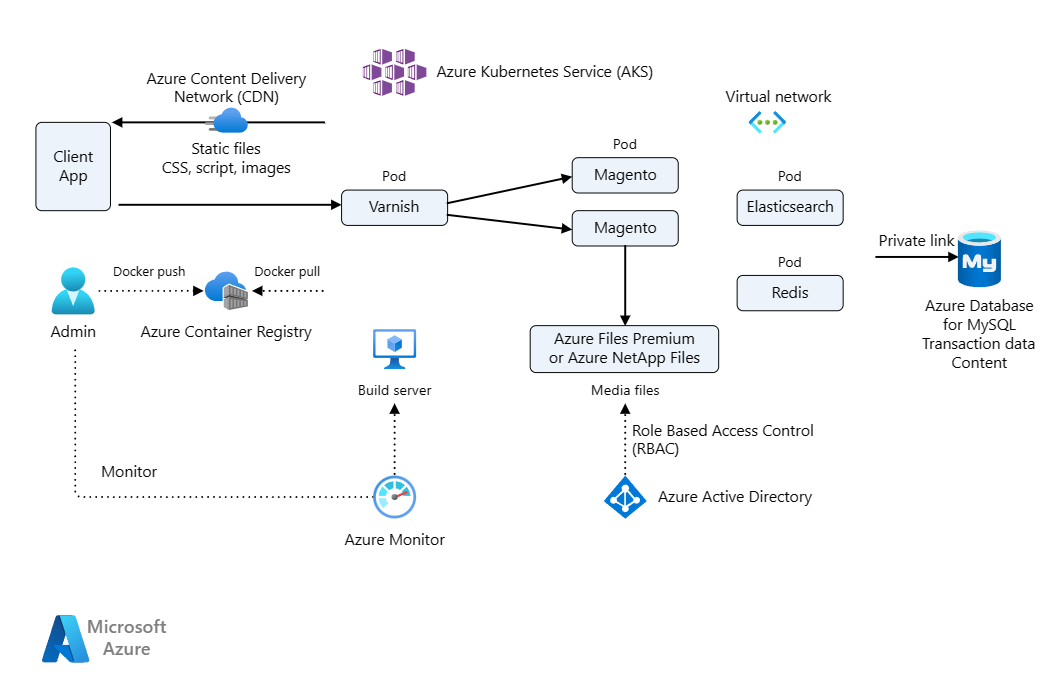
\includegraphics[scale=0.7]{images/hieu/chap-2/magento-architecture.png}
    \caption{Sơ đồ kiến trúc của Magento}
\end{figure}    
\subsubsection{Các thành phần của kiến trúc}
    \begin{itemize}
        \item \textbf{Azure Kubernetes Service (AKS)}: chia tỉ lệ các vùng chứa (containers) trên các dịch vụ mà Kubernetes quản lý.
        \item \textbf{Azure Virtual Network}: mạng ảo trên đám mây (cloud).
        \item \textbf{Azure Database for MySQL}: MySQL trên cloud giúp tiết kiệm chi phí, dễ thiết lập vận hành và mở rộng quy mô.
        \item \textbf{Azure Files}: chia sẻ các files trên cloud.
        \item \textbf{Azure NetApp Files}: chia sẻ các file Azure cấp doanh nghiệp, được cung cấp bởi NetApp.
        \item \textbf{Azure Content Delivery Network}: mạng phân phối nội dung nhanh chóng, đáng tin cậy và toàn cầu.
        \item \textbf{Microsoft Entra ID}: quản lý quyền try cập và định danh multicloud.
        \item \textbf{Azure Container Registry}: lưu trữ các hình ảnh vùng chứa riêng tư có thể chạy trong cụm AKS.
        \item \textbf{Azure Monitor}: thu thập và lưu trữ số liệu cũng như nhật ký, bao gồm dữ liệu đo từ xa của ứng dụng cũng như số liệu dịch vụ và nền tảng Azure.
    \end{itemize} 
\subsubsection{Workflow}
    \begin{itemize}
        \item Azure Kubernetes Service (AKS):triển khai Kubernetes bằng cách phân cụm thành các nhóm (pod) gồm Varnish, Magento, Redis và Elaticsearch.
        \item AKS tạo ra một mạng ảo (Virtual Network) để triển khai các node. Tạo trước mạng ảo để thiết lập cấu hình mạng con, liên kết riêng tư và hạn chế đầu ra. 
        \item Varnish cài đặt trước máy chủ HTTP để hoạt động như full-page cache (Full-page cache hay còn gọi là Cache toàn trang: Kỹ thuật này sẽ nén toàn bộ dữ liệu của website sang tệp HTML tĩnh và phản hồi cho trình duyệt khi được gọi).
        \item Cơ sở dữ liệu Azure cho MySQL lưu trữ dữ liệu giao dịch như đơn đặt hàng (Orders) và danh mục (catalogs) .
        \item Azure Files Premium, Azure NetApp Files hoặc hệ thống lưu trữ gắn mạng (Network-Attached Storage) tương đương lưu trữ các tệp phương tiện như hình ảnh sản phẩm. Magento cần một hệ thống tệp tương thích với Kubernetes có thể gắn ổ đĩa ở chế độ ReadWriteMany, như Azure Files Premium hoặc Azure NetApp Files. Lưu trữ các tuỳ chọn cho các ứng dụng trong Azure Kubernetes Service (AKS).
        \item Mạng phân phối nội dung (Content Delivery Network) phục vụ nội dung tĩnh như CSS, JavaScript và hình ảnh. Cung cấp nội dung thông qua CDN giảm thiểu độ trễ mạng giữa người dùng và trung tâm dữ liệu. CDN có thể loại bỏ tải đáng kể khỏi NAS bằng cách lưu vào bộ nhớ đệm và cung cấp nội dung tĩnh. 
        \item Redis lưu trữ session data. Nên lưu trữ Redis trên vùng chứa vì lý do hiệu suất. AKS sử dụng  Microsoft Entra ID để tạo và quản lý các tài nguyên Azure khác như bộ cân bằng tải Azure, xác thực người dùng, kiểm soát quyền truy cập dựa trên vai trò và danh tính được quản lý. 
        \item Azure Container Registry lưu trữ các hình ảnh Docker riêng được triển khai vào cụm AKS. Bạn có thể sử dụng các cơ quan đăng ký vùng chứa khác như Docker Hub. Cài đặt Magento mặc định ghi một số bí mật vào hình ảnh. 
        \item Azure Monitor thu thập và lưu trữ số liệu cũng như nhật ký, bao gồm số liệu nền tảng dịch vụ Azure và dữ liệu đo từ xa của ứng dụng. Azure Monitor tích hợp với AKS để thu thập số liệu bộ điều khiển, nút và bộ chứa cũng như nhật ký bộ chứa và nút chính.   
    \end{itemize}
\subsubsection{Khả năng mở rộng - scalability}
    \begin{itemize}
        \item \textbf{Media and static files}
            \begin{itemize}
                \item Cung cấp đầy đủ các files Azure, files Azure NetApp hoặc hệ thống lưu trữ gắn mạng (NAS) khác. Magento có thể lưu trữ hàng nghìn file media như hình ảnh sản phẩm. Đảm bảo cung cấp các sản phẩm NAS có tỉ lệ IOPS (Input/Outpur per Second) hợp lý để đáp ứng nhu cầu. 
                \item Giảm thiểu kích thước của nội dung tĩnh như HTML, CSS và JavaScript. Việc giảm thiểu có thể giảm chi phí băng thông và mang lại trải nghiệm phản hồi nhanh hơn cho người dùng. 
            \end{itemize}
        \item \textbf{Caching}: Cân bằng tải bộ đệm Varnish bằng cách chạy nhiều phiên bản trên các pods để có thể mở rộng quy mô.
        \item \textbf{Database Connection}: Bật kết nối liên tục với cơ sở dữ liệu MySQL, vì vật magento tiếp tục sử dụng lại kết nối hiện có thay vì tạo kết nối mới cho mọi yêu cầu.
        \item \textbf{Logging}: Hạn chế ghi nhật ký truy cập để tránh các vấn đề về hiệu suất và ngăn chặn việc lộ dữ liệu nhạy cảm như địa chỉ IP của khách hàng.  
    \end{itemize}
\subsubsection{Khả năng sẵn sàng phục vụ - availability}
    \begin{itemize}
        \item \textbf{Health Probes}: tương tự 2 case study được đề cập ở trên.
        \item \textbf{Availability Zones}
            \begin{itemize}
                \item Availability zones là các vị trí thực tế duy nhất trong  Azure regions giúp bảo vệ ứng dụng và dữ liệu khỏi lỗi của trung tâm dữ liệu. 
                \item Mỗi vùng được tạo thành từ một hoặc nhiều trung tâm dữ liệu. Các ứng dụng trong vùng có thể vẫn khả dụng ngay cả khi có lỗi vật lý trong một trung tâm dữ liệu. 
                \item Các cụm AKS có thể được triển khai trên nhiều Availability zones để cung cấp mức sẵn sàng cao hơn và bảo vệ khỏi các lỗi phần cứng hoặc các sự kiện bảo trì theo kế hoạch. Việc phân cụm các nhóm nodes để trải rộng trên nhiều vùng cho phép các nút tiếp tục hoạt động ngay cả khi một vùng duy nhất bị hỏng.  
            \end{itemize}
        \item \textbf{Resource constraints}
            \begin{itemize}
                \item Tranh chấp tài nguyên có thể ảnh hưởng đến tính sẵn có của dịch vụ. Xác định các ràng buộc về tài nguyên vùng chứa để không một vùng chứa nào có thể lấn át tài nguyên bộ nhớ cụm và CPU, có thể sử dụng chẩn đoán AKS để xác định bất kỳ vấn đề nào trong cụm.
                \item Sử dụng giới hạn tài nguyên để hạn chế tổng tài nguyên cho phép cho một vùng chứa, giúp cân bằng tài nguyên giữa các vùng chứa. 
            \end{itemize}
    \end{itemize}
\subsection{Giải pháp triển khai cho ứng dụng web về sản phẩm công nghệ trên AWS}
\noindent Tham khảo từ bài viết Scale Your Web Application — One Step at a Time của Saurabh Shrivastava.\footnote{Nguồn tham khảo: https://aws.amazon.com/vi/blogs/architecture/scale-your-web-application-one-step-at-a-time}

\subsubsection{Bối cảnh}
Giả sử chúng ta có một trang web tin tức công nghệ nơi chúng ta thực hiện đánh giá sơ bộ về đợt ra mắt điện thoại thông minh sắp ra mắt và rất được mong đợi, thông tin này đã lan truyền rộng rãi. Bài đánh giá, một bài đăng blog trên trang web của chúng ta, bao gồm cả video và hình ảnh. Tính năng bình luận được bật cho bài viết và người đọc cũng có thể đánh giá bài viết đó. 
\subsubsection{Giải pháp đề xuất}
\begin{figure}[H]
    \begin{center}
    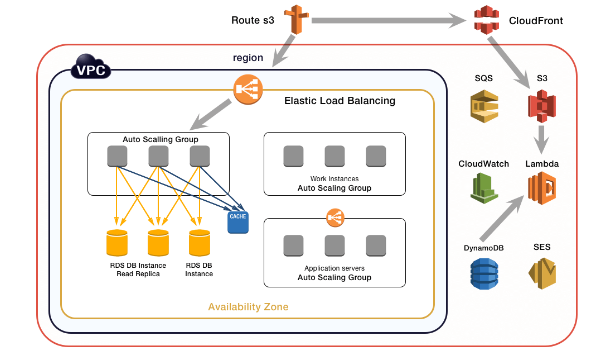
\includegraphics[scale=1]{images/hieu/chap-2/aws-architecture.png}
    \vspace*{5mm}
    \caption{AWS Architecture}
    \end{center}
\end{figure} 
\begin{itemize}
    \item \textbf{Bước 1: Load server dễ dàng}
        \newline
        Chúng ta cần nhanh chóng xử lý lưu lượng truy cập tăng đột biến, vì vậy, việc giảm tải máy chủ chúng ta chúng tag cách di chuyển hình ảnh và video sang một số mạng phân phối nội dung của bên thứ ba (CDN). \\[0.5cm]
        AWS cung cấp Amazon CloudFront dưới dạng giải pháp CDN, có khả năng mở rộng cao với tính năng bảo mật tích hợp để xác minh danh tính truy cập nguồn gốc và xử lý mọi cuộc tấn công DDoS. \\[0.5cm]
        CloudFront có thể hướng lưu lượng truy cập đến máy chủ local hoặc được lưu trữ trên cloud.
    \item \textbf{Bước 2: Giảm read request bằng cách thêm nhiều read replicas}
        \begin{figure}[H]
            \begin{center}
            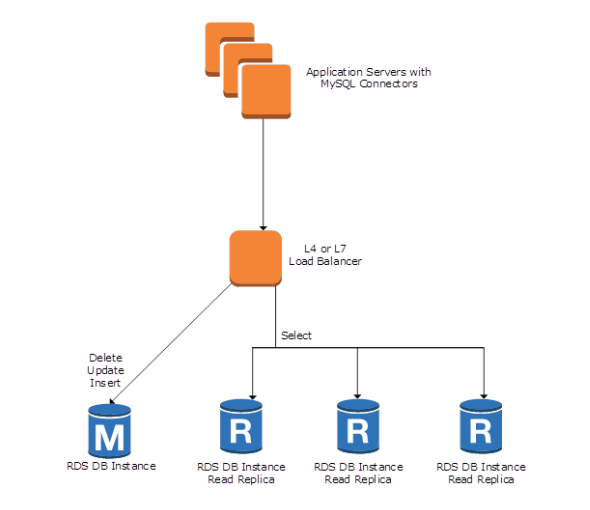
\includegraphics[scale=1]{images/hieu/chap-2/read-replica.png}
            \vspace*{5mm}
            \caption{Tăng số lượng read replicas}
            \end{center}
        \end{figure} 
    \item \textbf{Bước 3: Giảm write request}
        \begin{figure}[H]
            \begin{center}
            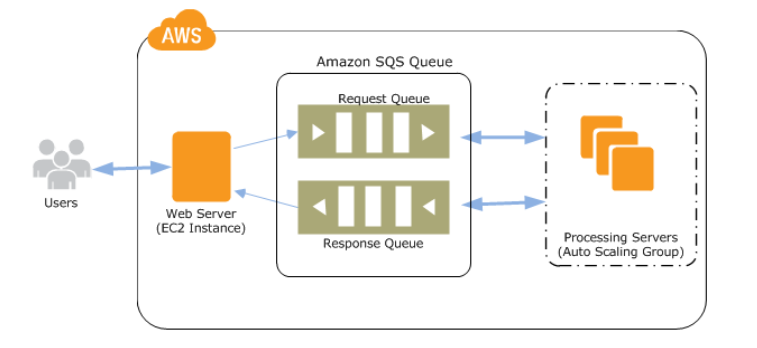
\includegraphics[scale=0.8]{images/hieu/chap-2/write-request-1.png}
            \vspace*{5mm}
            \caption{Amazon Simple Queue Service}
            \end{center}
        \end{figure}

        \begin{figure}[H]
            \begin{center}
            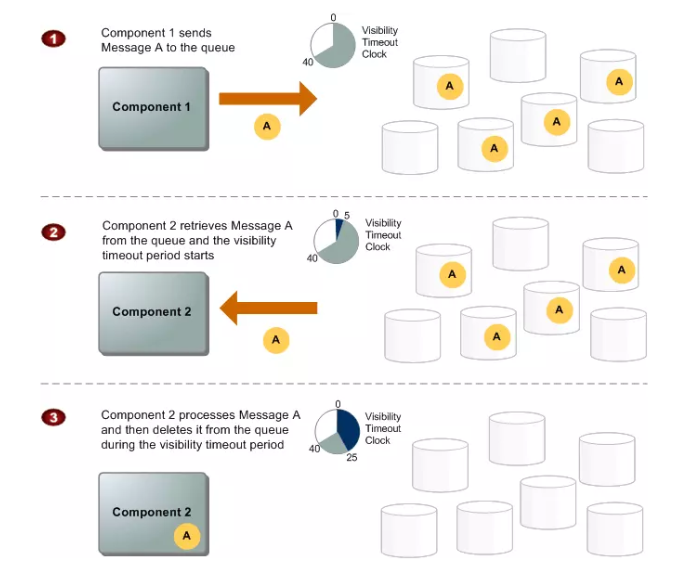
\includegraphics[scale=0.8]{images/hieu/chap-2/write-request-2.png}
            \vspace*{5mm}
            \caption{Giảm write request}
            \end{center}
        \end{figure}
        Điều này có thể đạt được bằng cách đưa vào hàng đợi để xử lý thông báo không đồng bộ. Amazon Simple Queue Service (Amazon SQS) là hàng đợi có khả năng mở rộng cao, có thể xử lý mọi loại tải tin nhắn công việc. chúng ta có thể xử lý dữ liệu, như xếp hạng và đánh giá.
    \item \textbf{Bước 4: Amazon Elasticache}
    \newline
        Chúng ta có thể sử dụng Amazon Elasticache cho Memcached hoặc Redis để giảm yêu cầu ghi. Memcached và Redis có các trường hợp sử dụng khác nhau, vì vậy nếu chúng ta có đủ khả năng để mất và khôi phục bộ đệm từ cơ sở dữ liệu của mình, hãy sử dụng Memcached.\\[0.5cm]
        Nếu chúng ta đang tìm kiếm tính bền vững của dữ liệu mạnh mẽ hơn và cấu trúc dữ liệu phức tạp hơn, hãy sử dụng Redis. Trong AWS, đây là những dịch vụ được quản lý, nghĩa là AWS sẽ đảm nhận khối lượng công việc cho chúng ta và chúng ta cũng có thể triển khai chúng trong các phiên bản tại chỗ của mình hoặc sử dụng phương pháp kết hợp.
    \item  \textbf{Bước 5: Mở rộng quy mô máy chủ}
    \newline
    Nếu vẫn còn sự cố, đã đến lúc mở rộng quy mô máy chủ. Để có hiệu quả chi phí cao nhất và khả năng mở rộng không giới hạn, chúng ta nên luôn sử dụng tỷ lệ theo chiều ngang (horizontal scaling).\\[0.5cm]
    Nếu máy chủ của chúng ta đặt tại chỗ (on promise), thì nên cân nhắc việc tạo kiến trúc nhiều trang, điều này sẽ giúp chúng ta đạt được khả năng mở rộng nhanh chóng theo yêu cầu và cung cấp giải pháp khắc phục thảm họa tốt, chúng ta có thể chọn các dịch vụ riêng lẻ như Amazon Route 53, AWS CloudFormation, Amazon SQS, Amazon SNS, Amazon RDS, v.v. tùy theo nhu cầu của chúng ta.\\[0.5cm]
    Kiến trúc multi-site của chúng ta sẽ trông giống như sơ đồ sau:
    \begin{figure}[H]
        \begin{center}
        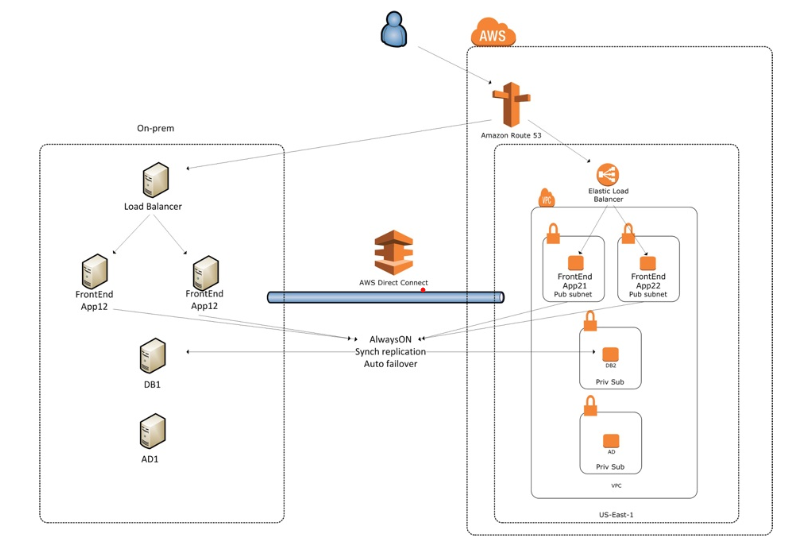
\includegraphics[scale=0.8]{images/hieu/chap-2/multi-site-architecture.png}
        \vspace*{5mm}
        \caption{Kiến trúc multi-site}
        \end{center}
    \end{figure}
        Trong kiến trúc này, chúng ta có thể chạy khối lượng công việc thông thường của mình tại on-premise và sử dụng khối lượng công việc AWS theo yêu cầu để có khả năng mở rộng và khắc phục thảm họa. chúng tag cách sử dụng Route 53, chúng ta có thể hướng một tỷ lệ phần trăm người dùng chính xác tới khối lượng công việc AWS.\\[0.5cm]
        Nếu chúng ta quyết định chuyển tất cả khối lượng công việc của mình sang AWS, kiến trúc multi-AZ được đề xuất sẽ như sau:
        \begin{figure}[H]
            \begin{center}
            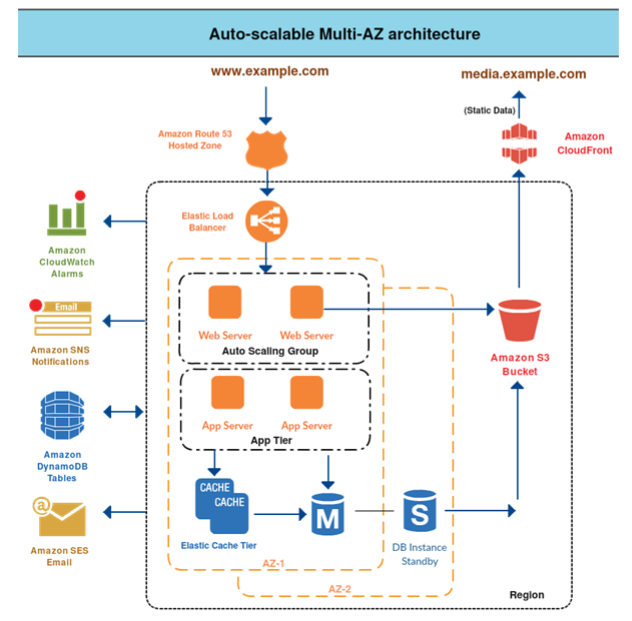
\includegraphics[scale=0.8]{images/hieu/chap-2/multi-AZ-architecture.png}
            \vspace*{5mm}
            \caption{Kiến trúc multi-AZ}
            \end{center}
        \end{figure}
        Đối với kiểu kiến trúc này, chúng ta đang sử dụng khối lượng công việc phân tán nhiều AZ để có tính sẵn sàng cao. chúng ta có thể thiết lập nhiều AZ và sử dụng Route 53 để phân bổ khối lượng công việc của mình giữa các Khu vực AWS.\\[0.5cm]
        CloudFront giúp chúng ta mở rộng quy mô và phân phối nội dung tĩnh thông qua bộ chứa S3 và DynamoDB, duy trì trạng thái ứng dụng của chúng ta để Tự động chia tỷ lệ có thể áp dụng tỷ lệ theo chiều ngang (Horizontal) mà không làm mất dữ liệu. Ở lớp cơ sở dữ liệu, RDS với chế độ chờ multi-AZ cung cấp tính sẵn sàng cao và chúng ta sao chỉ có quyền đọc giúp đạt được khả năng mở rộng.\\[0.5cm]
        Chúng ta nên tạo một mô hình kết hợp, nhiều địa điểm bằng cách đặt bản sao môi trường tại chỗ trên đám mây công cộng như Đám mây AWS, đồng thời sử dụng Dịch vụ DNS Amazon Route53 và 
        Elastic Load Balancing để định tuyến lưu lượng giữa môi trường tại chỗ (on premise) và đám mây (cloud).\\[0.5cm]
        AWS hiện hỗ trợ cân bằng tải giữa AWS và môi trường tại chỗ để giúp chúng ta mở rộng môi trường đám mây một cách nhanh chóng, bất cứ khi nào cần và giảm thiểu hơn nữa bằng cách áp dụng khả năng tự động thay đổi quy mô của Amazon và đặt ngưỡng cho lưu lượng truy cập tại chỗ của chúng ta bằng Route 53.
    \end{itemize}
\subsection{Phân tích ảnh hưởng của các framework PHP khi triển khai ứng dụng trên EKS}
\noindent Tham khảo từ bài viết "Scaling PHP Applications on AWS" của ADRIANO CATALUDDI.\protect\footnote{Nguồn tham khảo: https://www.logicata.com/blog/scaling-php-applications-on-aws}
\subsubsection{Bối cảnh}
    Trước khi chúng ta bắt đầu mở rộng quy mô của một ứng dụng PHP lên trên cloud, điều quan trọng là phải tuân theo các biện pháp liên quan đến hiệu suất và phương pháp phát triển. Tối ưu hóa hiệu suất rất quan trọng vì tắc nghẽn hiệu suất ở cấp độ hard code sẽ cản trở chúng ta khi thực hiện các cải tiến đối với cơ sở hạ tầng AWS.\\[0.5cm]
    Thực tiễn phát triển tốt rất quan trọng để đảm bảo rằng chúng ta có sự cân bằng phù hợp giữa tốc độ phát triển, mức độ dễ đọc của code và tính linh hoạt trong ứng dụng của mình.\\[0.5cm]
    Ngoài việc đảm bảo rằng chúng ta có mã tối ưu và các phương pháp phát triển tốt thì việc nên hiểu một số lợi ích và hạn chế của việc lựa chọn framework PHP trước khi chuẩn bị mở rộng quy mô của ứng dụng.\\[0.5cm]
    Các framework giúp chúng ta không phải đưa ra các quyết định quan trọng về kiến trúc cho dự án của mình, nhưng chúng ta có thể phải trả giá vì việc không cân nhắc khi sử dụng chúng. Lợi ích chính của hầu hết các framework bao gồm các đoạn code mạnh mẽ hơn, nhiều chức năng vượt trội hơn và tốc độ phát triển nhanh hơn.\\[0.5cm]
    Tuy nhiên, cái giá phải trả khi sử dụng framework là chúng thường có các mẫu kiến trúc cố định và tính không linh hoạt này có thể dẫn đến khó khăn khi sau này chúng ta muốn tích hợp ứng dụng của mình với AWS.\\[0.5cm]
    Với những sự cân bằng này, điều quan trọng là phải chọn framework nào bạn sẽ sử dụng nếu có và nó sẽ tác động như thế nào đến các quyết định mở rộng quy mô của chúng ta sau này. Các framework PHP phổ biến nhất là CodeIgniter, Symfony và Laravel.
\subsubsection{Tích hợp các framework PHP với kiến trúc phân tán}
    \begin{itemize}
        \item \textbf{CodeIgniter MVC architecture}
        \newline
        Mô hình ứng dụng của chúng ta có thể chứa những thứ như phiên người dùng (session) và bộ nhớ đệm (cache), do đó nó có thể gây khó khăn nếu những thứ này bị ràng buộc chặt chẽ với ứng dụng của chúng ta, vì điều này có nghĩa là chúng cũng bị ràng buộc với các phiên bản EC2 duy nhất của chúng ta. Điều này gây khó khăn nếu sau này chúng ta muốn mở rộng quy mô thành nhiều phiên bản EC2.
        \item \textbf{Symfony MVC architecture}
        \newline
        Symfony là một framework giúp phát triển các thành phần tách rời và một khung MVC tùy chọn được triển khai trên các thành phần này. Điều này đặc biệt có lợi khi tích hợp với AWS vì chúng ta vẫn có thể duy trì tính linh hoạt trong kiến trúc trong khi vẫn tận dụng được các thành phần của Symfony, được thiết kế để thực hiện các tác vụ phát triển dễ dàng hơn.
        \item \textbf{Laravel MVC architecture}
        \newline
        Laravel là một framework thường sử dụng kiến trúc MVC để phát triển ứng dụng, nghĩa là có thể cần nhiều bước hơn để tách các phần khác nhau trong ứng dụng của chúng ta thành các service khác nhau trên AWS. Tuy nhiên, Laravel có khả năng tùy biến cao (option cao) nên vẫn có nhiều lựa chọn để mở rộng quy mô trên AWS với Laravel.\\[0.5cm]
        Một lựa chọn khác là không sử dụng framework nào cả. Điều này cho phép linh hoạt tối đa vì có toàn quyền kiểm soát kiến trúc của mình và có thể phát triển kiến trúc phân tán tương thích hơn với AWS ngay từ đầu.
    \end{itemize}
\subsection{Giải pháp triển khai cho ứng dụng microservice trên EKS}
\noindent Tham khảo từ bài viết"Microservices Deployment on EKS" của STACKSIMPLIFY.\footnote{Nguồn tham khảo: https://www.stacksimplify.com/aws-eks/microservices-on-aws-eks/learn-to-deploy-microservices-on-aws-eks}
\subsubsection{Bối cảnh}
Chúng ta sẽ triển khai hai microservice:
\begin{itemize}
    \item Quản lý người dùng: tạo API người dùng sẽ gọi service.
    \item Thông báo: gửi API thông báo để gửi email cho người dùng khi chúng ta tạo một tài khoản người dùng mới.
\end{itemize}
\begin{figure}[H]
    \begin{center}
    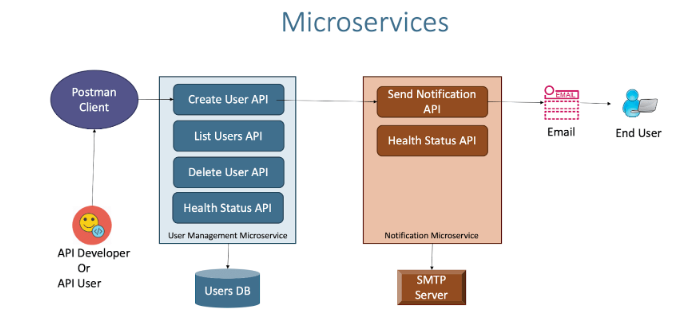
\includegraphics[scale=1]{images/hieu/chap-2/microservice.png}
    \vspace*{5mm}
    \caption{Hai microservices quản lý người dùng và thông báo}
    \end{center}
\end{figure}
\subsubsection{Kiến trúc giải pháp}
Sơ đồ kiến trúc được triển khai như hình:
\begin{figure}[H]
    \begin{center}
    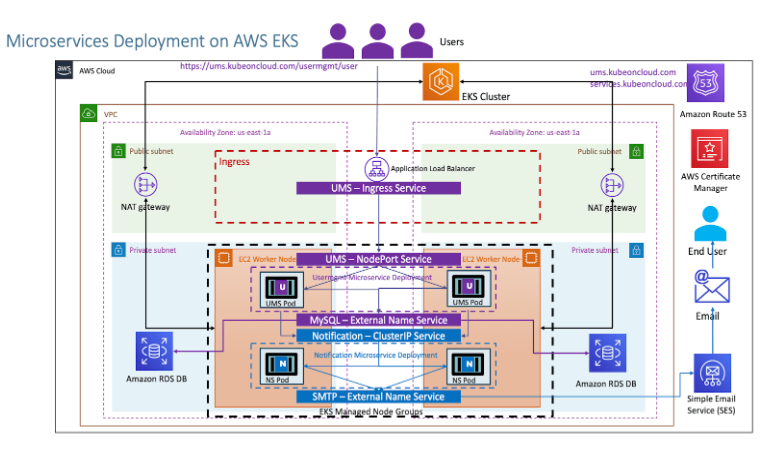
\includegraphics[scale=0.8]{images/hieu/chap-2/solution-architecture.png}
    \vspace*{5mm}
    \caption{Sơ đồ iến trúc giải pháp}
    \end{center}
\end{figure}    
Khi có request từ Users hướng đến hệ thống, các request sẽ được phân tán ra 02 availability zone - nơi đặt các máy chủ của hệ thống thông qua một service của AWS là Ingress Service, sau đó request được dẫn đến các EC2 Worker Node nơi chứa các pods của hệ thống để xử lý logic (Amazon RDS DB để lưu dữ liệu của ứng dụng, Amazon Route 53 để phân giải tên miền) cho các request đó, sau đó thông báo sẽ được gửi đến người dùng thông qua service khác của EKS có tên là Simple Email Service (SES).
\chapter{Phân tích yêu cầu}
\section{Phân tích yêu cầu nghiệp vụ}
\subsection{Yêu cầu chức năng}
Hệ thống có một số tính năng chính sau:
\begin {list} {-}{}
    \item Người dùng có thể đăng ký tài khoản cho riêng mình.
    \item Người dùng có thể đăng nhập vào hệ thống với tài khoản và mật khẩu đã đăng ký thành công trước đó.
    \item Người dùng có thể đổi mật khẩu khi cần thiết.
    \item Khi truy cập và hệ thống, người dùng có thể xem được tất cả các sản phẩm của cửa hàng.
    \item Hệ thống có thể phân loại sản phẩm theo từng loại khác nhau.
    \item Người dùng có thể tìm kiếm sản phẩm theo tên, loại, giá, kích thước\dots
    \item Người dùng có thể xem chi tiết sản phẩm để lựa chọn được sản phẩm phù hợp nhất.
    \item Người dùng có thể thêm sản phẩm vào giỏ hàng.
    \item Người dùng có thể xem giỏ hàng của mình.
    \item Người dùng có thể xóa sản phẩm, điều chỉnh số lượng sản phẩm trong giỏ hàng.
    \item Người dùng có thể xem tổng số tiền hiện tại của giỏ hàng.
    \item Người dùng có thể thanh toán những sản phẩm trong giỏ hàng bằng nhiều hình thức khác nhau như: tiền mặt, thẻ tín dụng, ví điện tử\dots
    \item Người dùng có thể xem lịch sử mua hàng của mình.
    \item Người dùng có thể để lại những đánh giá về sản phẩm mà mình đã mua.
    \item Hệ thống phân quyền người dùng theo từng vai trò khác nhau gồm có: khách hàng (customer), nhân viên (staff), quản lý (manager).
    \item Khi đăng nhập với vai trò là nhân viên, người dùng có thể thêm, sửa, xóa, điều chỉnh sản phẩm và quản lý đơn hàng.
    \item Khi đăng nhập với vai trò là quản lý, người dùng có thể thêm, sửa, xóa, điều chỉnh sản phẩm, quản lý đơn hàng, và quản lý người dùng sử dụng hệ thống (thêm, sửa, xóa, chặn\dots).
    \item Hệ thống thống kê doanh thu thành biểu đồ theo từng ngày,tháng,năm để nhân viên và quản lý có thể dễ dàng theo dõi.
\end {list}
\subsection{Yêu cầu phi chức năng}
Hệ thống có một số yêu cầu phi chức năng như sau:
\begin {list} {-}{}
    \item Hệ thống có giao diện thân thiện với người dùng.
    \item Hệ thống có thể dễ dàng sử dụng đối với người dùng mới.
    \item Hệ thống có thể hoạt động tốt trên hầu hết các trình duyệt hiện nay như Chrome, Firefox, Safari, Microsoft Edge\dots
    \item Hệ thống hoạt động tốt trên nhiều loại thiết bị khác nhau như máy tính, điện thoại, máy tính bảng\dots
    \item Hệ thống có thể chạy mượt mà, ổn định.
    \item Hệ thống có thể chịu tải tốt, phục vụ nhiều người dùng cùng một lúc.
    \item Hệ thống phục vụ người dùng 24/7.
    \item Hệ thống có thể bảo mật thông tin người dùng bằng những phương pháp mã hoá thông tin nhạy cảm.
\newpage
\section{Phân tích hệ thống}
\subsection{Use case diagram}
\subsubsection{Use case diagram cho toàn bộ tính năng của hệ thống}
\begin{figure}[H]
    \begin{center}
    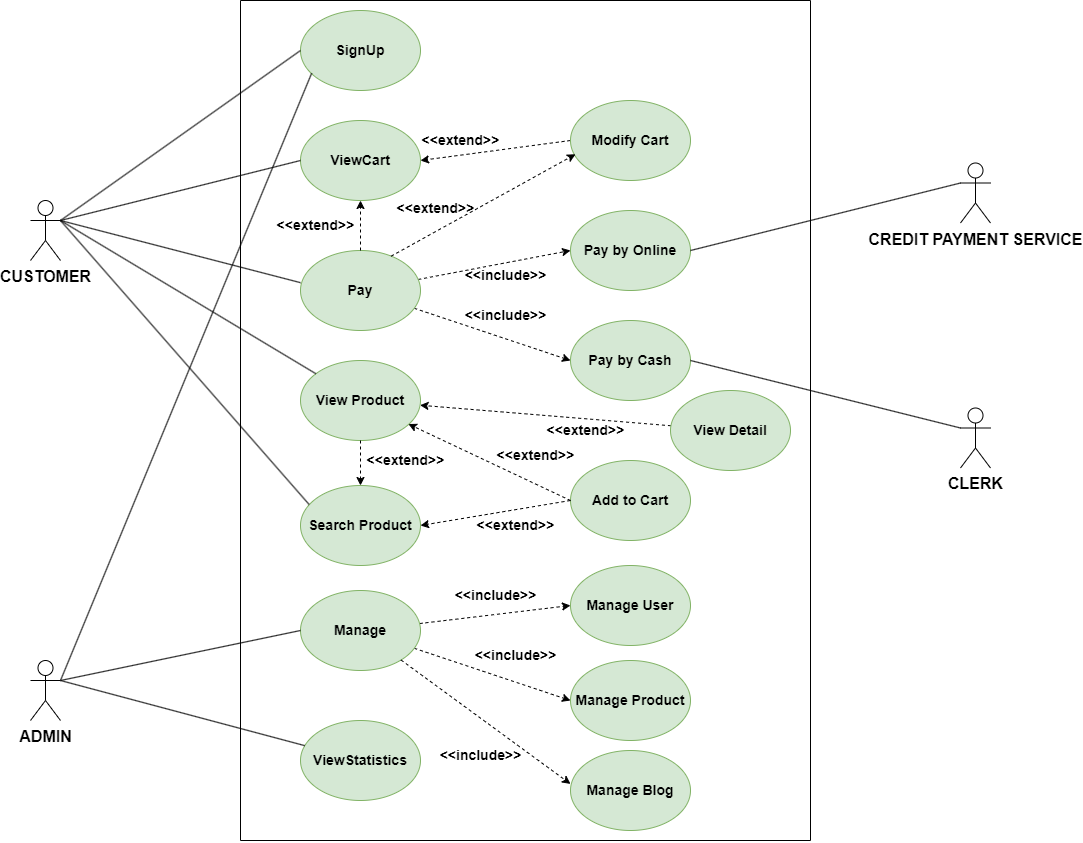
\includegraphics[scale=0.45]{images/hieu/chap-3/usecase-diagram.png}
    \vspace*{5mm}
    \caption{Use case diagram cho toàn bộ tính năng của hệ thống}
    \end{center}
\end{figure}
\newpage
\subsubsection{Đặc tả use case cho một số tính năng chính}
\begin{itemize}
    \item \textbf{Đăng nhập}
    \begin{table}[H]
        \begin{tabular}{|l|l|}
        \hline
        \textbf{Use-case name}    & \textbf{Đăng nhập - Login}                                                                                                                                                                                                                                                                                                                                                                                                                           \\ \hline
        \textbf{Actor}            & User (Manager, Customer, Staff)                                                                                                                                                                                                                                                                                                                                                                                                                      \\ \hline
        \textbf{Description}      & Người dùng đăng nhập vào hệ thống                                                                                                                                                                                                                                                                                                                                                                                                                    \\ \hline
        \textbf{Pre-condition}    & Người dùng đã đăng ký tài khoản thàng công                                                                                                                                                                                                                                                                                                                                                                                                           \\ \hline
        \textbf{Post-condition}   & Người dùng đăng nhập thành công                                                                                                                                                                                                                                                                                                                                                                                                                      \\ \hline
        \textbf{Normal-flow}      & \begin{tabular}[c]{@{}l@{}}1.Người dùng chọn biểu tượng đăng nhập trên góc phải màn hình.\\ 2.Hệ thống hiển thị trang đăng nhập.\\ 3.Người dùng nhập thông tin đã đăng ký gồm tên người dùng (username) và \\ mật khẩu (password)\\ 4.Người dùng chọn nút "ĐĂNG NHẬP".\\ 5.1.Hệ thống chuyển đến "TRANG CHỦ" nếu xác thực thông tin thành công.\\ 5.2.Nếu thông tin sai, hệ thống yêu cầu người dùng nhập lại.\\ 6.Đăng nhập thành công\end{tabular} \\ \hline
        \textbf{Alternative-flow} & Không có                                                                                                                                                                                                                                                                                                                                                                                                                                             \\ \hline
        \textbf{Exception}        & \begin{tabular}[c]{@{}l@{}}Nếu người dùng bị chặn bởi người quản lý (Manager) sẽ không thể đăng nhập \\ vào hệ thống\end{tabular}                                                                                                                                                                                                                                                                                                                    \\ \hline
        \end{tabular}
        \begin{center}
            Bảng 3.1: Đặc tả use case đăng nhập
        \end{center}
        \end{table}
        
    \item \textbf{Đăng ký}
    \begin{table}[H]
        \begin{tabular}{|l|l|}
        \hline
        \textbf{Use-case name}    & \textbf{Đăng ký - SignUp}                                                                                                                                                                                                                                                                                                                                                                                                                                                                                                                              \\ \hline
        \textbf{Actor}            & User (Manager, Customer, Staff)                                                                                                                                                                                                                                                                                                                                                                                                                                                                                                                        \\ \hline
        \textbf{Description}      & Người dùng đăng ký tài khoản để truy cập vào hệ thống                                                                                                                                                                                                                                                                                                                                                                                                                                                                                                  \\ \hline
        \textbf{Pre-condition}    & Người dùng truy cập vào website thành công                                                                                                                                                                                                                                                                                                                                                                                                                                                                                                             \\ \hline
        \textbf{Post-condition}   & Người dùng đăng ký tài khoản thành công                                                                                                                                                                                                                                                                                                                                                                                                                                                                                                                \\ \hline
        \textbf{Normal-flow}      & \begin{tabular}[c]{@{}l@{}}1.Người dùng chọn biểu tượng đăng nhập trên góc phải màn hình.\\ 2.Hệ thống hiển thị trang đăng nhập.\\ 3.Người dùng nhấn vào liên kết "Bạn chưa có tài khoản?" \\ 4.Hệ thống chuyển sang trang đăng ký tài khoản.\\ 5.Người dùng nhập đầy đủ thông tin mà hệ thống yêu cầu như họ tên, email,\\ địa chỉ, số điện thoại...\\ 6.Chọn nút "ĐĂNG KÝ"\\ 7.1.Hệ thống hiển thị đăng ký thành công \\ 7.2.Hệ thống yêu cầu nhập lại thông tin nếu có sai sót (thiếu trường thông tin,\\ email không thể xác thực...) \\8.Hệ thống lưu thông tin người dùng.\end{tabular} \\ \hline
        \textbf{Alternative-flow} & Không có                                                                                                                                                                                                                                                                                                                                                                                                                                                                                                                                               \\ \hline
        \textbf{Exception}        & Một địa chỉ email chỉ đăng ký được một tài khoản.                                                                                                                                                                                                                                                                                                                                                                                                                                                                                                      \\ \hline
        \end{tabular}
        \begin{center}
            Bảng 3.2: Đặc tả use case đăng ký tài khoản
        \end{center}
    \end{table}
    \newpage
    \item \textbf{Xem sản phẩm}
    \begin{table}[H]
        \begin{tabular}{|l|l|}
        \hline
        \textbf{Use-case name}    & \textbf{Xem sản phẩm - View Products}                                                                                                                                                                                                                                                                                                                                                                                                                                                                                                                                                                                                                                                                                                                                                                           \\ \hline
        \textbf{Actor}            & User (Manager, Customer, Staff)                                                                                                                                                                                                                                                                                                                                                                                                                                                                                                                                                                                                                                                                                                                                                                                 \\ \hline
        \textbf{Description}      & Người dùng xem những sản phẩm được bày bán trên cửa hàng                                                                                                                                                                                                                                                                                                                                                                                                                                                                                                                                                                                                                                                                                                                                                        \\ \hline
        \textbf{Pre-condition}    & Người dùng đăng nhập vào hệ thống thành công                                                                                                                                                                                                                                                                                                                                                                                                                                                                                                                                                                                                                                                                                                                                                                     \\ \hline
        \textbf{Post-condition}   & Người dùng có thể xem sản phẩm của cửa hàng                                                                                                                                                                                                                                                                                                                                                                                                                                                                                                                                                                                                                                                                                                                                                                     \\ \hline
        \textbf{Normal-flow}      & \begin{tabular}[c]{@{}l@{}}1.Người dùng truy cập vào website.\\ 2.Hệ thống tự động chuyển đến trang chủ (HomePage).\\ 3.Tại trang chủ, người dùng có thể lướt để xem tất cả những sản phẩm được   \\ hiển thị theo loại, ngoài ra còn có những sản phẩm nổi bật, những sản phẩm\\ sắp được ra mắt trong tương lai.\\ 4.Người dùng có thể tìm kiếm sản phẩm mình muốn bằng cách nhập từ khoá \\ (tên, loại, giá, kích thước...) vào ô tìm kiếm rồi nhấn nút "TÌM KIẾM".\\ 5.Hệ thống hiển thị kết quả tìm kiếm.\\ 6.Người dùng nhấn vào từng sản phẩm \\ 7.Hệ thống hiển thị thông tin chi tiết của sản phẩm tương ứng.\\ 8.Nếu người dùng muốn mua sản phẩm:\\       8.1.Nhấn vào nút "MUA HÀNG" để trực tiếp mua sản phẩm.\\       8.2.Nhấn vào biểu tưởng giỏ hàng để thêm sản phẩm vào giỏ hàng.\end{tabular} \\ \hline
        \textbf{Alternative-flow} & Không có                                                                                                                                                                                                                                                                                                                                                                                                                                                                                                                                                                                                                                                                                                                                                                                                        \\ \hline
        \textbf{Exception}        & Người dùng phải đăng nhập mới có thể mua hàng hoặc thêm vào giỏ hàng.                                                                                                                                                                                                                                                                                                                                                                                                                                                                                                                                                                                                                                                                                                                                                                                                        \\ \hline
        \end{tabular}
        \begin{center}
            Bảng 3.3: Đặc tả use case xem sản phẩm
        \end{center}
        \end{table}
        
        \item \textbf{Quản lý giỏ hàng}
        \begin{table}[H]
            \begin{tabular}{|l|l|}
            \hline
            \textbf{Use-case name}    & \textbf{Quản lý giỏ hàng - Cart Manager}                                                                                                                                                                                                                                 \\ \hline
            \textbf{Actor}            & User (Manager, Customer, Staff)                                                                                                                                                                                                                                          \\ \hline
            \textbf{Description}      & Người dùng quản lý giỏ hàng của mình                                                                                                                                                                                                                                     \\ \hline
            \textbf{Pre-condition}    & Người dùng đăng nhập vào hệ thống thành công                                                                                                                                                                                                                             \\ \hline
            \textbf{Post-condition}   & Người dùng quản lý giỏ hàng thành công                                                                                                                                                                                                                                   \\ \hline
            \textbf{Normal-flow}      & \begin{tabular}[c]{@{}l@{}}1.Người dùng nhấn vào biểu tượng giỏ hàng nằm trên thanh điều hướng.\\ 2.Hệ thống hiển thị chi tiết trang giỏ hàng.\\ 3.Tại đây, người dùng có thể.\\ -Thêm / Xoá sản phẩm khỏi giỏ hàng.\\ -Tăng / Giảm số lượng từng sản phẩm.\end{tabular} \\ \hline
            \textbf{Alternative-flow} & Không có                                                                                                                                                                                                                                                                 \\ \hline
            \textbf{Exception}        & Không có                                                                                                                                                                                                                                                                 \\ \hline
            \end{tabular}
            \begin{center}
                Bảng 3.4: Đặc tả use case quản lý giỏ hàng
            \end{center}
            \end{table}
        \newpage
        \item \textbf{Thanh toán}
            \begin{table}[H]
                \begin{tabular}{|l|l|}
                \hline
                \textbf{Use-case name}    & \textbf{Thanh toán - Payment}                                                                                                                                                                                                                                                                                                                                                                                                                                                                                                                                                                                                                                                                                                                                                                                                              \\ \hline
                \textbf{Actor}            & User (Manager, Customer, Staff), Credit Payment Service                                                                                                                                                                                                                                                                                                                                                                                                                                                                                                                                                                                                                                                                                                                                                                                    \\ \hline
                \textbf{Description}      & Người dùng thanh toán đơn hàng của mình                                                                                                                                                                                                                                                                                                                                                                                                                                                                                                                                                                                                                                                                                                                                                                                                    \\ \hline
                \textbf{Pre-condition}    & Người dùng đăng nhập vào hệ thống thành công                                                                                                                                                                                                                                                                                                                                                                                                                                                                                                                                                                                                                                                                                                                                                                                               \\ \hline
                \textbf{Post-condition}   & Người dùng thanh toán thành công                                                                                                                                                                                                                                                                                                                                                                                                                                                                                                                                                                                                                                                                                                                                                                                                           \\ \hline
                \textbf{Normal-flow}      & \begin{tabular}[c]{@{}l@{}}1.Người dùng nhấn vào biểu tượng giỏ hàng nằm trên thanh điều hướng.\\ 2.Hệ thống hiển thị chi tiết trang giỏ hàng.\\ 3.Tại giỏ hàng, người dùng có thể chọn lại những sản phẩm cần mua ngay.\\ 4.Chọn nút "THANH TOÁN".\\ 5.Hệ thống tính toán tổng số tiền cần trả (bao gồm cả phí vận chuyển) rồi\\ hiển thị lên màn hình.\\ 6.Người dùng lựa chọn phương thức thanh toán:\\ 6.1.Thanh toán tiền mặt: Người dùng để lại thông tin, đơn hàng sẽ được\\ tổng hợp và người dùng có thể ra cửa hàng để thanh toán.\\ 6.2.Thanh toán bẳng thẻ tín dụng, thẻ ngân hàng, ví điện tử:\\ -Người dùng chọn dịch vụ phù hợp.\\ -Dịch vụ bên thứ 3 sẽ liên kết và xử lý thanh toán.\\ -6.2.1.Hệ thống thông báo thanh toán thành công.\\ -6.2.2.Hệ thống thông báo lỗi, yêu cầu người dùng thực hiện lại.\end{tabular} \\ \hline
                \textbf{Alternative-flow} & Không có                                                                                                                                                                                                                                                                                                                                                                                                                                                                                                                                                                                                                                                                                                                                                                                                                                   \\ \hline
                \textbf{Exception}        & Không có                                                                                                                                                                                                                                                                                                                                                                                                                                                                                                                                                                                                                                                                                                                                                                                                                                   \\ \hline
                \end{tabular}
                \begin{center}
                    Bảng 3.5: Đặc tả use case thanh toán
                \end{center}
                \end{table}
                
        \item \textbf{Quản lý sản phẩm}
            \begin{table}[H]
                \begin{tabular}{|l|l|}
                \hline
                \textbf{Use-case name}    & \textbf{Quản lý sản phẩm - Products Manager}                                                                                                                                                                                                                                                                                                                                                                                                                                                                                                                                                                                                                                        \\ \hline
                \textbf{Actor}            & Manager, Staff                                                                                                                                                                                                                                                                                                                                                                                                                                                                                                                                                                                                                                                                      \\ \hline
                \textbf{Description}      & Người quản lý và nhân viên quản lý sản phẩm của cửa hàng                                                                                                                                                                                                                                                                                                                                                                                                                                                                                                                                                                                                                            \\ \hline
                \textbf{Pre-condition}    & Người dùng đăng nhập vào hệ thống với vai trò là quản lý hoặc nhân viên                                                                                                                                                                                                                                                                                                                                                                                                                                                                                                                                                                                                             \\ \hline
                \textbf{Post-condition}   & Người dùng quản lý sản phẩm thành công.                                                                                                                                                                                                                                                                                                                                                                                                                                                                                                                                                                                                                                             \\ \hline
                \textbf{Normal-flow}      & \begin{tabular}[c]{@{}l@{}}1.Tại trang web, người dùng chọn nút "SẢN PHẨM".\\ 2.Hệ thống chuyển đến trang quản lý sản phẩm.\\ 3.Tại đây, người dùng có thể thấy tất cả các sản phẩm hiện có cũng như những\\ thông tin chi tiết của chúng.\\ 4.1.Người dùng có thể nhấn "CHỈNH SỬA" để điều chỉnh thông tin sản phẩm\\ 4.2.Người dùng có thể nhấn "THÊM" để thêm sản phẩm mới\\ -4.2.1.Hệ thống hiện thị một popup để người dùng thêm sản phẩm mới\\ -4.2.2.Người dùng nhập thông tin cần thiết cho sản phẩm mới\\ -4.2.3.Người dùng chọn "THÊM" để xác nhận \\ 4.3.Người dùng chọn "XOÁ" để xoá sản phẩm khỏi hệ thống\\ 5.Hệ thống lưu lại hành động của người dùng.\end{tabular} \\ \hline
                \textbf{Alternative-flow} & Không có                                                                                                                                                                                                                                                                                                                                                                                                                                                                                                                                                                                                                                                                            \\ \hline
                \textbf{Exception}        & Không có                                                                                                                                                                                                                                                                                                                                                                                                                                                                                                                                                                                                                                                                            \\ \hline
                \end{tabular}
                \begin{center}
                    Bảng 3.6: Đặc tả use case quản lý sản phẩm
                \end{center}
                \end{table}
            \newpage
            \item \textbf{Quản lý người dùng}
            \begin{table}[H]
            \begin{tabular}{|l|l|}
            \hline
            \textbf{Use-case name}    & \textbf{Quản lý người dùng - User Manager}                                                                                                                                                                                                                                                                                                                                                                                                                                                                                                                                                                                              \\ \hline
            \textbf{Actor}            & Manager                                                                                                                                                                                                                                                                                                                                                                                                                                                                                                                                                                                                                                 \\ \hline
            \textbf{Description}      & Người quản lý quản lý những người sử dụng hệ thống                                                                                                                                                                                                                                                                                                                                                                                                                                                                                                                                                                                      \\ \hline
            \textbf{Pre-condition}    & Người dùng đăng nhập vào hệ thống với vai trò là quản lý                                                                                                                                                                                                                                                                                                                                                                                                                                                                                                                                                                                \\ \hline
            \textbf{Post-condition}   & Manager quản lý người dùng thành công                                                                                                                                                                                                                                                                                                                                                                                                                                                                                                                                                                                                   \\ \hline
            \textbf{Normal-flow}      & \begin{tabular}[c]{@{}l@{}}1.Hệ thống chuyển sang trang quản lý.\\ 2.Manager chọn "NGƯỜI DÙNG"\\ 3.Hệ thống hiển thị tất cả người dùng của trang web.\\ 4.Tại đây, manager có thể:\\ 4.1.Thêm người dùng mới vào hệ thống bằng cách chọn nút "THÊM"\\ 4.2.Xoá người dùng khỏi hệ thống bằng cách chọn nút "XOÁ" nằm bên cạnh \\ người dùng cần xoá.\\ 4.3.Điều chỉnh thông tin người dùng bằng cách chọn nút "ĐIỀU CHỈNH"\\ 4.4.Chặn không cho người dùng tiếp tục sử dụng trang web bằng cách chọn \\ nút "CHẶN".\\ 4.5.Bỏ chặn người dùng bằng cách chọn nút "BỎ CHẶN"\\ 5.Hệ thống lưu lại hành động của người quản lý.\end{tabular} \\ \hline
            \textbf{Alternative-flow} & Không có                                                                                                                                                                                                                                                                                                                                                                                                                                                                                                                                                                                                                                \\ \hline
            \textbf{Exception}        & Không có                                                                                                                                                                                                                                                                                                                                                                                                                                                                                                                                                                                                                                \\ \hline
            \end{tabular}
            \begin{center}
                Bảng 3.7: Đặc tả use case quản lý người dùng
            \end{center}
            \end{table}
            \item \textbf{Xem thống kê doanh thu}
            \begin{table}[H]
                \begin{tabular}{|l|l|}
                \hline
                \textbf{Use-case name}    & \textbf{Xem thống kê doanh thu - View Statistic}                                                                                                                                                                                                                                                                                                                                 \\ \hline
                \textbf{Actor}            & Manager                                                                                                                                                                                                                                                                                                                                                                          \\ \hline
                \textbf{Description}      & Người quản lý có thể xem doanh thu của cửa hàng                                                                                                                                                                                                                                                                                                                                  \\ \hline
                \textbf{Pre-condition}    & Người dùng đăng nhập vào hệ thống với vai trò là quản lý                                                                                                                                                                                                                                                                                                                         \\ \hline
                \textbf{Post-condition}   & Manager xem doanh thu thành công                                                                                                                                                                                                                                                                                                                                                 \\ \hline
                \textbf{Normal-flow}      & \begin{tabular}[c]{@{}l@{}}1.Hệ thống chuyển sang trang quản lý.\\ 2.Manager chọn nút "THỐNG KÊ"\\ 3.Hệ thống chuyển sang trang thống kê\\ 4.Tại trang thống kê, người quản lý chọn khoảng thời gian và chọn sản phẩm \\ \\ (có thể xem thống kê của một hoặc nhiều loại sản phẩm)\\ 5.Hệ thống hiển thi thống kê dưới dạng các biểu đồ.\\ 6.Hoàn tất xem thống kê.\end{tabular} \\ \hline
                \textbf{Alternative-flow} & Không có                                                                                                                                                                                                                                                                                                                                                                         \\ \hline
                \textbf{Exception}        & Không có                                                                                                                                                                                                                                                                                                                                                                         \\ \hline
                \end{tabular}
                \begin{center}
                    Bảng 3.8: Đặc tả use case xem thống kê doanh thu
                \end{center}
                \end{table}
    \end{itemize}
\newpage
\subsection{Activity diagram}
\subsubsection{Activity diagram cho user là khách hàng}
\begin{figure}[H]
    \centering
    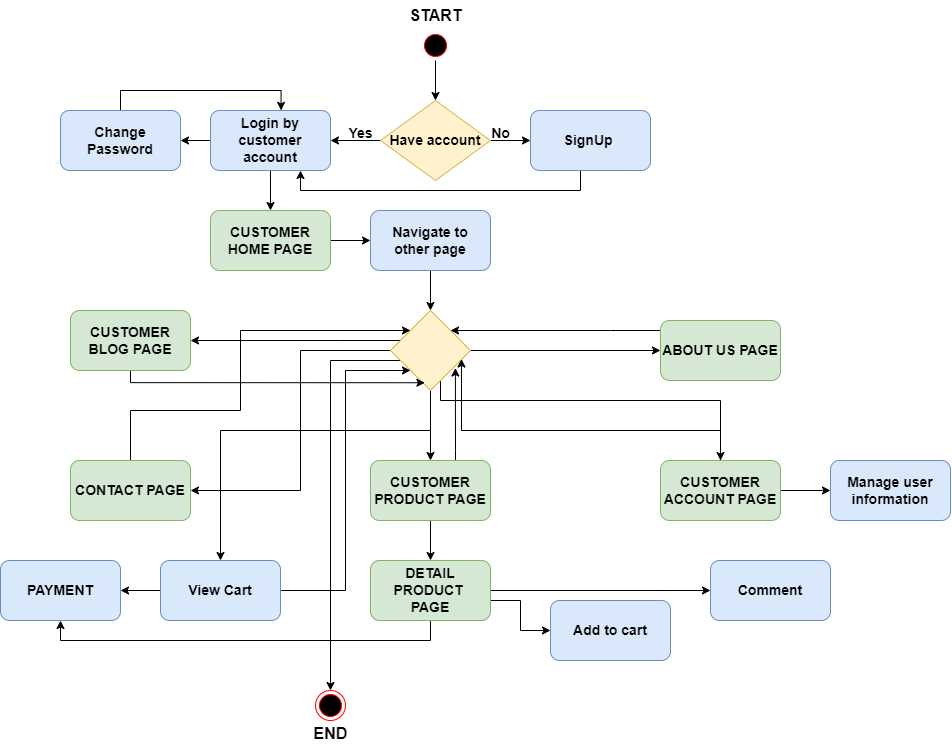
\includegraphics[scale=0.45]{images/hieu/chap-3/user-activity-diagram.png}
    \caption{Activity diagram cho user là khách hàng}
\end{figure}

\newpage
\subsubsection{Activity diagram cho user là quản lý}
\begin{figure}[H]
    \centering
    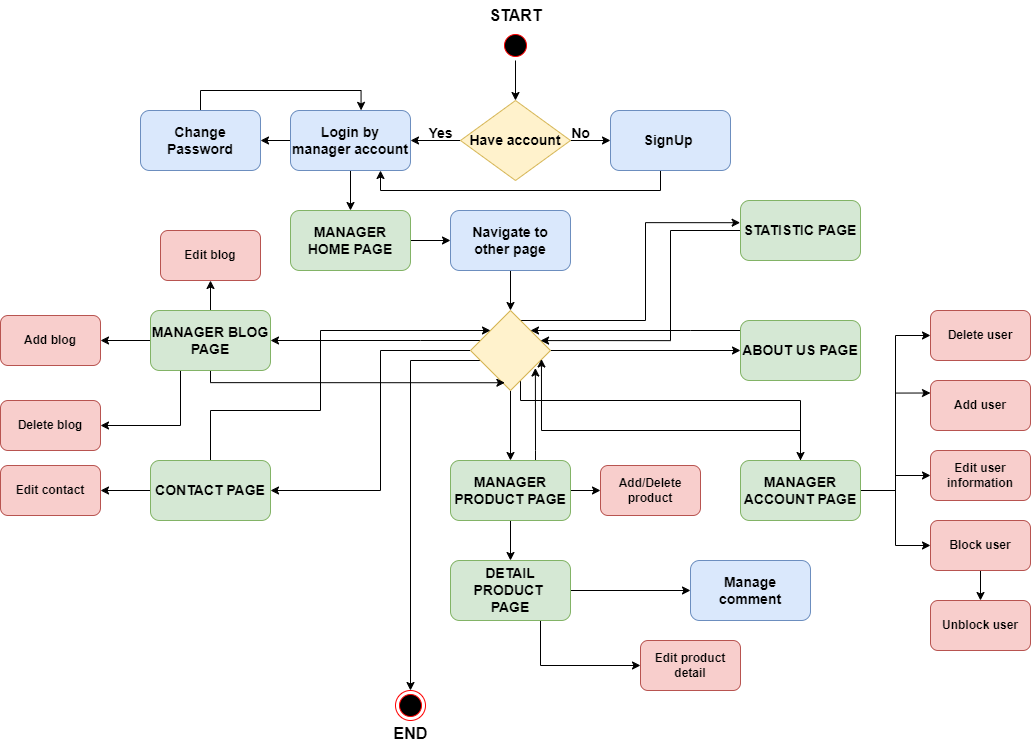
\includegraphics[scale=0.4]{images/hieu/chap-3/admin-activity-diagram.png}
    \caption{Activity diagram cho user là quản lý}
\end{figure}
\newpage
\subsubsection{Activity diagram cho chức năng đăng nhập - đăng ký}
\begin{figure}[H]
    \centering
    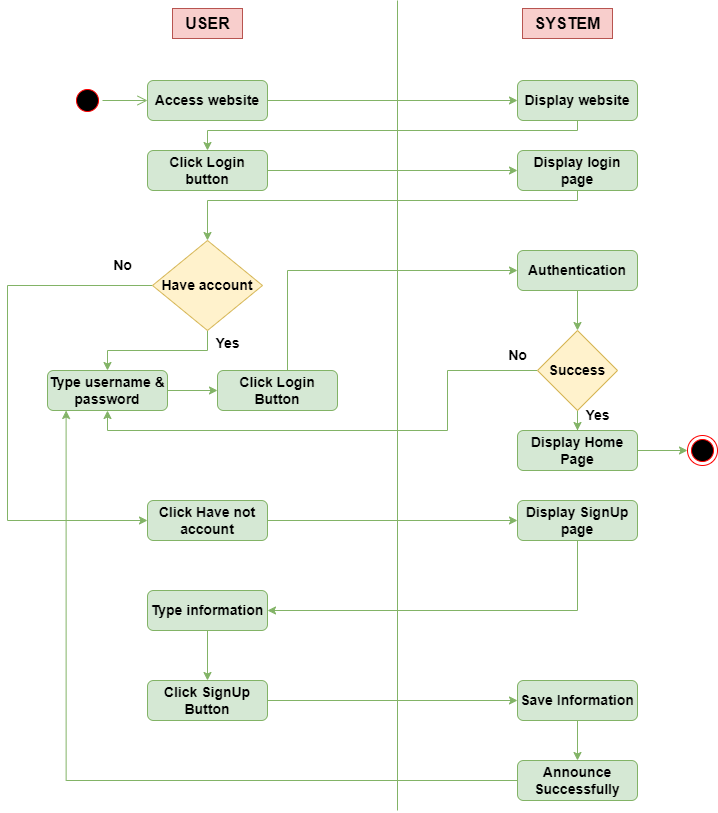
\includegraphics[scale=0.6]{images/hieu/chap-3/login-signup-activity-diagram.png}
    \caption{Activity diagram cho chức năng đăng nhập - đăng ký}
\end{figure}
\newpage
\subsubsection{Activity diagram cho chức năng quản lý}
\begin{figure}[H]
    \centering
    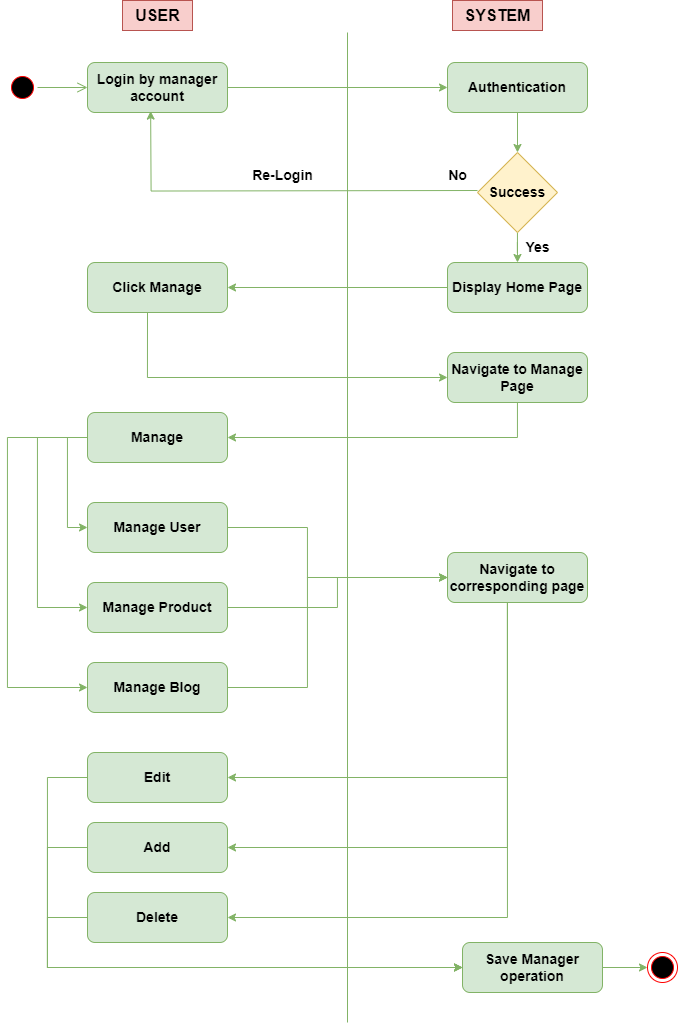
\includegraphics[scale=0.5]{images/hieu/chap-3/manage-activity-diagram.png}
    \caption{Activity diagram cho chức năng quản lý}
\end{figure}
\newpage
\subsubsection{Activity diagram cho chức năng mua sắm}
\begin{figure}[H]
    \centering
    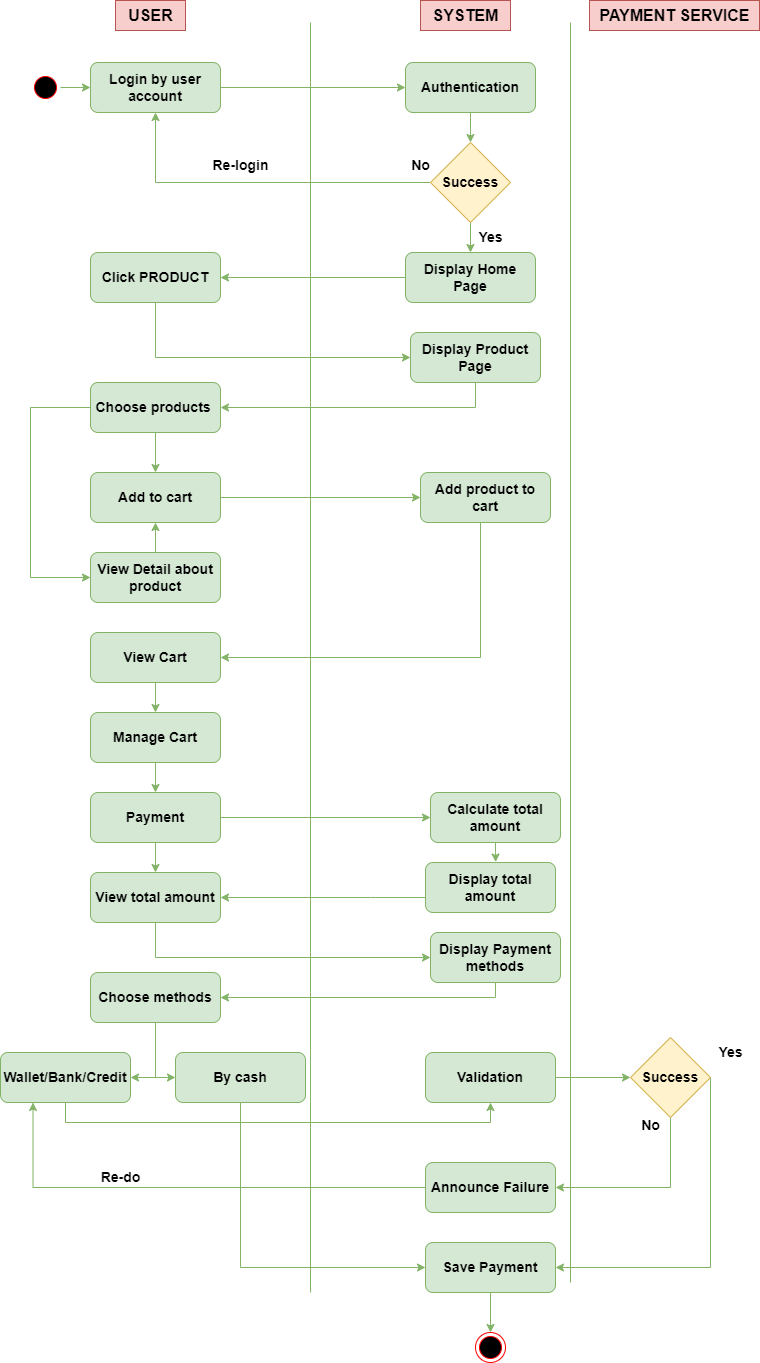
\includegraphics[scale=0.4]{images/hieu/chap-3/shopping-activity-diagram.png}
    \caption{Activity diagram cho chức năng mua sắm}
\end{figure}
\newpage
\subsubsection{Activity diagram cho chức năng xem thống kê}
\begin{figure}[H]
    \centering
    \includegraphics[scale=0.6]{images/hieu/chap-3/Statistic-activity-diagram.png}
    \caption{Activity diagram cho chức năng xem thống kê}
\end{figure}
\newpage
\subsection{Sequence diagram}
\subsubsection{Sequence diagram cho chức năng đăng nhập - đăng ký}
\begin{figure}[H]
    \centering
    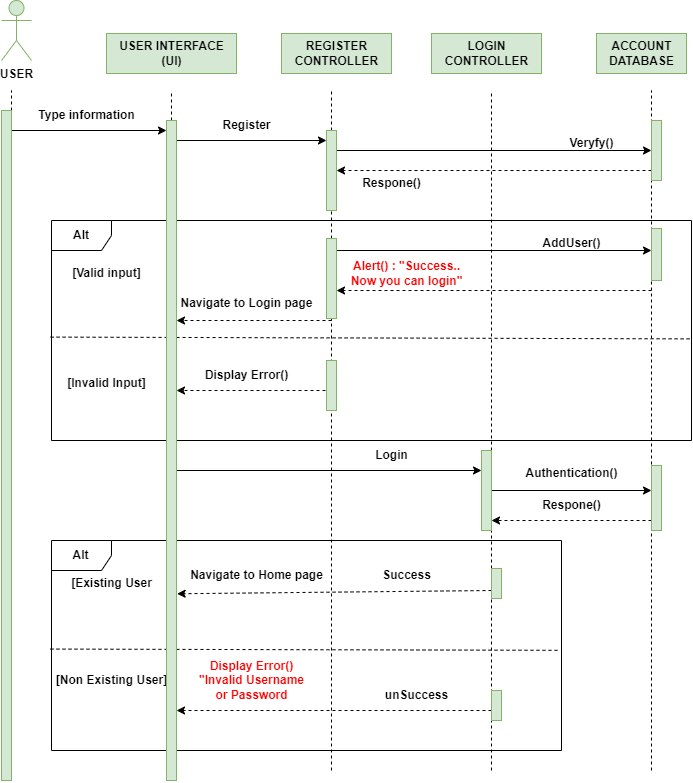
\includegraphics[scale=0.6]{images/hieu/chap-3/login-signup-sequence-diagram.png}
    \caption{Sequence diagram cho chức năng đăng nhập - đăng ký}
\end{figure}
Trong đó:
\begin{itemize}
    \item User: người dùng (khách hàng, quản lý, nhân viên) đăng ký tài khoản và đăng nhập vào hệ thống.
    \item User Interface: giao diện trang đăng nhập và trang đăng ký tương tác với người dùng.
    \item Rigister Controller: khối xử lý chức năng đăng ký tài khoản của người dùng.
    \item Login Controller: khối xử lý chức năng đăng nhập của người dùng.
    \item Account Database: cơ sở dữ liệu lưu thông tin tài khoản của người dùng.
\end{itemize}
\newpage
\subsubsection{Sequence diagram cho chức năng mua sắm}
\begin{figure}[H]
    \centering
    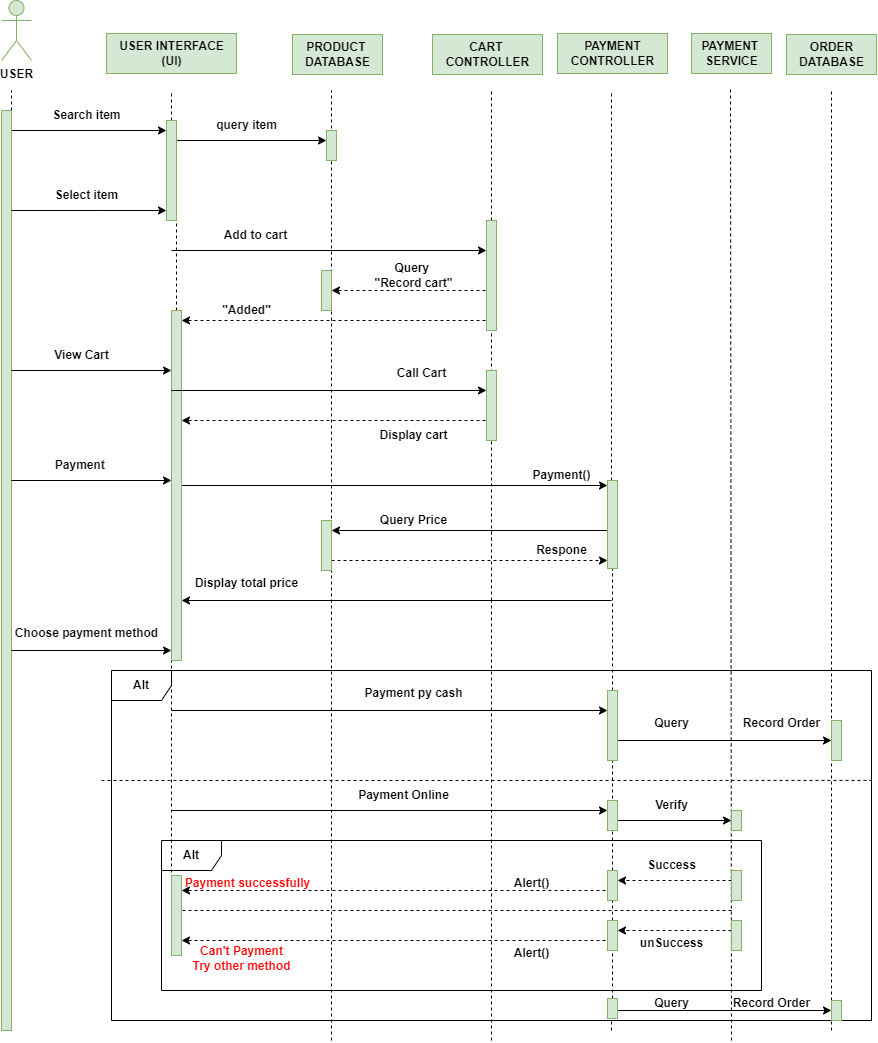
\includegraphics[scale=0.5]{images/hieu/chap-3/shopping-sequence-diagram.png}
    \caption{Sequence diagram cho chức năng mua sắm}
\end{figure}
Trong đó:
\begin{itemize}
    \item UserInterface: giao diện trang chủ, trang chi tiết sản phẩm, trang giỏ hàng và trang thanh toán tương tác với người dùng.
    \item Product Database: cơ sở dữ liệu lưu thông tin sản phẩm của cửa hàng.
    \item Cart Controller: khối xử lý chức năng quản lý giỏ hàng của người dùng.
    \item Payment Controller: khối xử lý chức năng thanh toán của người dùng.
    \item Payment Serice: dịch vụ thanh toán bên thứ 3.
    \item Order Database: cơ sở dữ liệu lưu thông tin đơn hàng của cửa hàng.
\end{itemize}
\newpage
\subsubsection{Sequence diagram cho chức năng quản lý sản phẩm}
\begin{figure}[H]
    \centering
    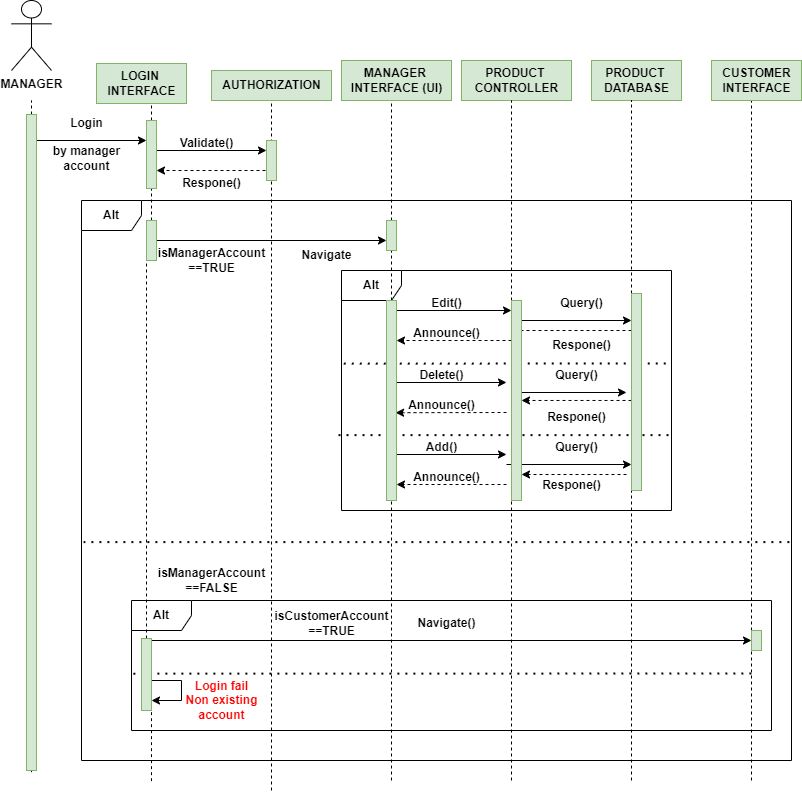
\includegraphics[scale=0.5]{images/hieu/chap-3/manage-product-sequence-diagram.png}
    \caption{Sequence diagram cho chức năng quản lý sản phẩm}
\end{figure}
Trong đó:
\begin{itemize}
    \item Manager: là người quản lý, sẽ quản lý tất cả các sản phẩm của cửa hàng.
    \item LoginInterface: giao diện trang đăng nhập tương tác với người dùng.
    \item Authorization: khối xử lý chức năng xác thực người dùng có phải là người quản lý hay không.
    \item Manager Interface: giao diện trang quản lý sản phẩm tương tác với người dùng.
    \item Product Controller: khối xử lý chức năng quản lý sản phẩm của người dùng.
    \item Product Database: cơ sở dữ liệu lưu thông tin sản phẩm của cửa hàng.
    \item Customer Interface: giao diện trang chủ tương tác với người dùng là khách hàng (trong trường hợp người dùng không phải là người quản lý).
\end{itemize}
\newpage
\subsubsection{Sequence diagram cho chức năng quản lý tài khoản}
\begin{figure}[H]
    \centering
    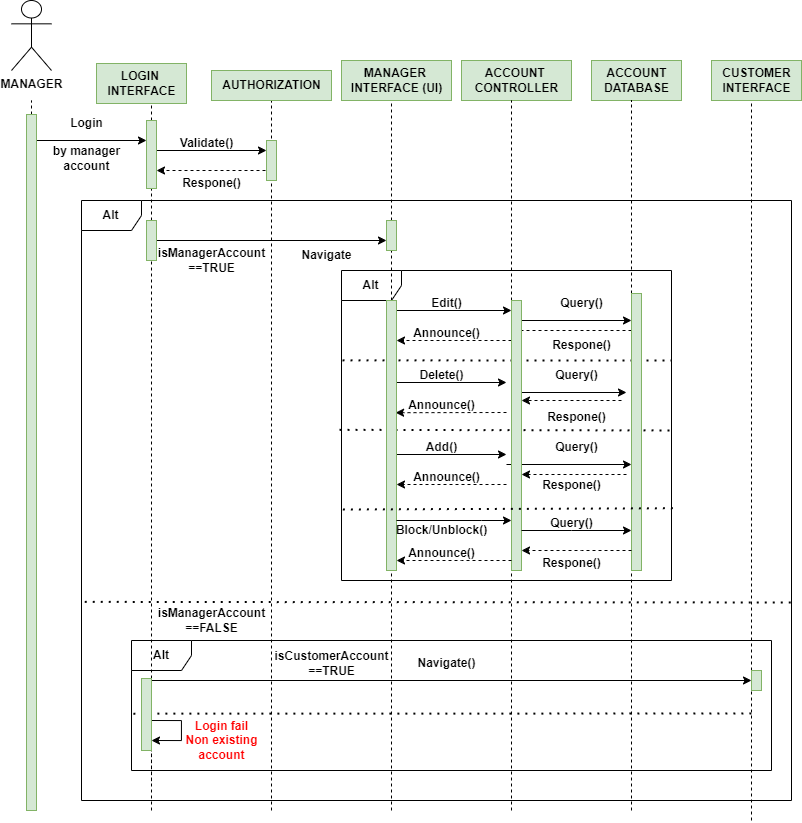
\includegraphics[scale=0.5]{images/hieu/chap-3/manage-account-sequence-diagram.png}
    \caption{Sequence diagram cho chức năng quản lý tài khoản}
\end{figure}
Trong đó:
\begin{itemize}
    \item Manager: là người quản lý, sẽ quản lý tất cả các sản phẩm của cửa hàng.
    \item LoginInterface: giao diện trang đăng nhập tương tác với người dùng.
    \item Authorization: khối xử lý chức năng xác thực người dùng có phải là người quản lý hay không.
    \item Manager Interface: giao diện trang quản lý tài khoản tương tác với người dùng.
    \item Account Controller: khối xử lý chức năng quản lý tài khoản của người dùng.
    \item Account Database: cơ sở dữ liệu lưu thông tin tài khoản của cửa hàng.
    \item Customer Interface: giao diện trang chủ tương tác với người dùng là khách hàng (trong trường hợp người dùng không phải là người quản lý).
\end{itemize}
\newpage
\subsubsection{Sequence diagram cho chức năng quản lý bài viết}
\begin{figure}[H]
    \centering
    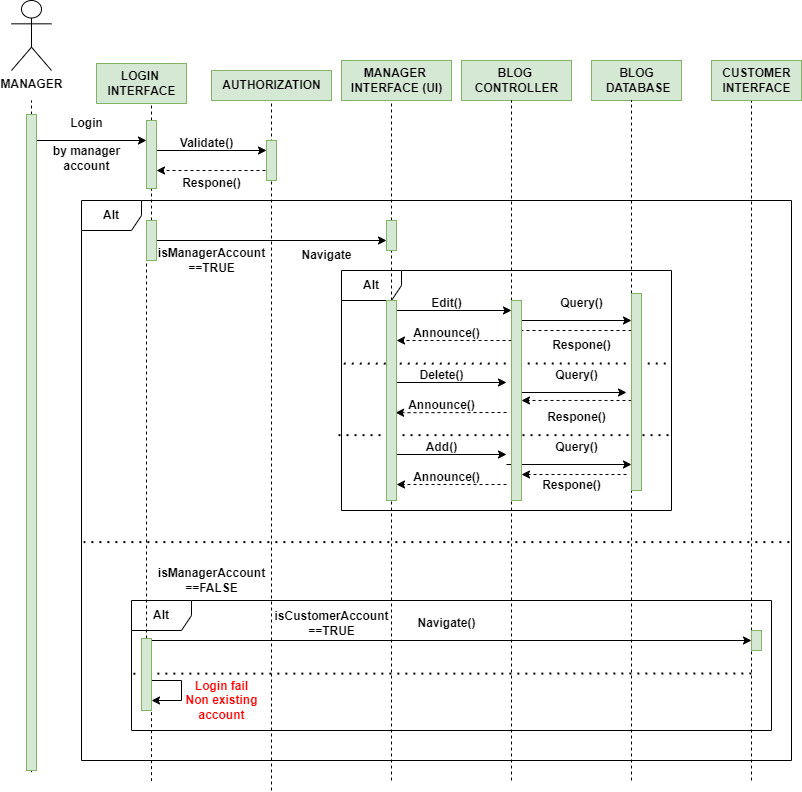
\includegraphics[scale=0.5]{images/hieu/chap-3/manage-blog-sequence-diagram.png}
    \caption{Sequence diagram cho chức năng quản lý bài viết}
\end{figure}
Trong đó:
\begin{itemize}
    \item Manager: là người quản lý, sẽ quản lý tất cả các sản phẩm của cửa hàng.
    \item LoginInterface: giao diện trang đăng nhập tương tác với người dùng.
    \item Authorization: khối xử lý chức năng xác thực người dùng có phải là người quản lý hay không.
    \item Manager Interface: giao diện trang quản lý bài viết tương tác với người dùng.
    \item Blog Controller: khối xử lý chức năng quản lý bài viết của người dùng.
    \item Blog Database: cơ sở dữ liệu lưu thông tin bài viết của cửa hàng.
    \item Customer Interface: giao diện trang chủ tương tác với người dùng là khách hàng (trong trường hợp người dùng không phải là người quản lý).
\end{itemize}
\newpage
\subsubsection{Sequence diagram cho chức năng xem thống kê doanh thu}
\begin{figure}[H]
    \centering
    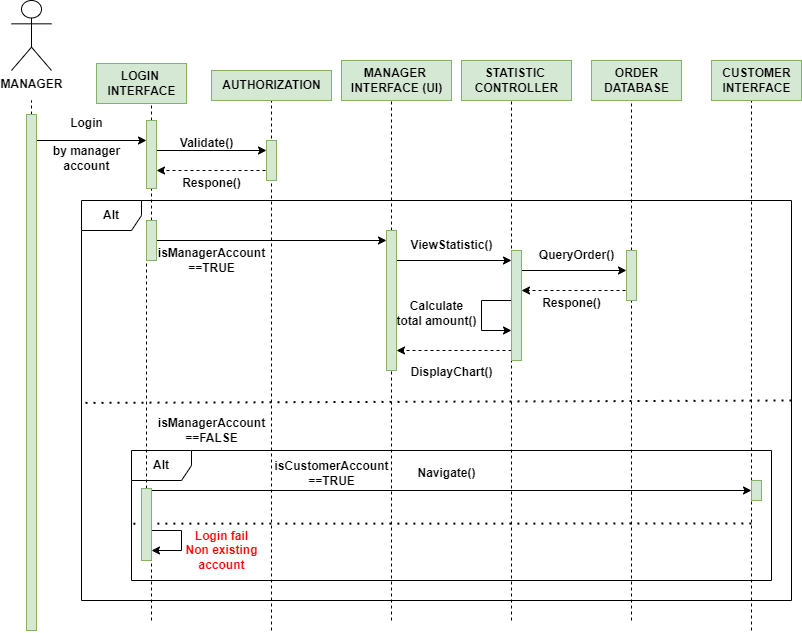
\includegraphics[scale=0.5]{images/hieu/chap-3/statistic-sequence-diagram.png}
    \caption{Sequence diagram cho chức năng xem thống kê doanh thu}
\end{figure}
Trong đó:
\begin{itemize}
    \item Manager: là người quản lý, sẽ quản lý tất cả các sản phẩm của cửa hàng.
    \item LoginInterface: giao diện trang đăng nhập tương tác với người dùng.
    \item Authorization: khối xử lý chức năng xác thực người dùng có phải là người quản lý hay không.
    \item Manager Interface: giao diện trang quản lý doanh thu tương tác với người dùng.
    \item Statistic Controller: khối xử lý chức năng xem thống kê doanh thu của người dùng.
    \item Order Database: cơ sở dữ liệu lưu thông tin đơn hàng của cửa hàng.
    \item Customer Interface: giao diện trang chủ tương tác với người dùng là khách hàng (trong trường hợp người dùng không phải là người quản lý).
\end{itemize}
\newpage
\subsection{Database diagram}
\subsubsection {Entity Relationship Diagram - ERD}
\textbf{Ghi chú:} Đây chỉ là sơ đồ cho chức năng liên quan đến sản phẩm
\begin{figure}[H]
    \centering
    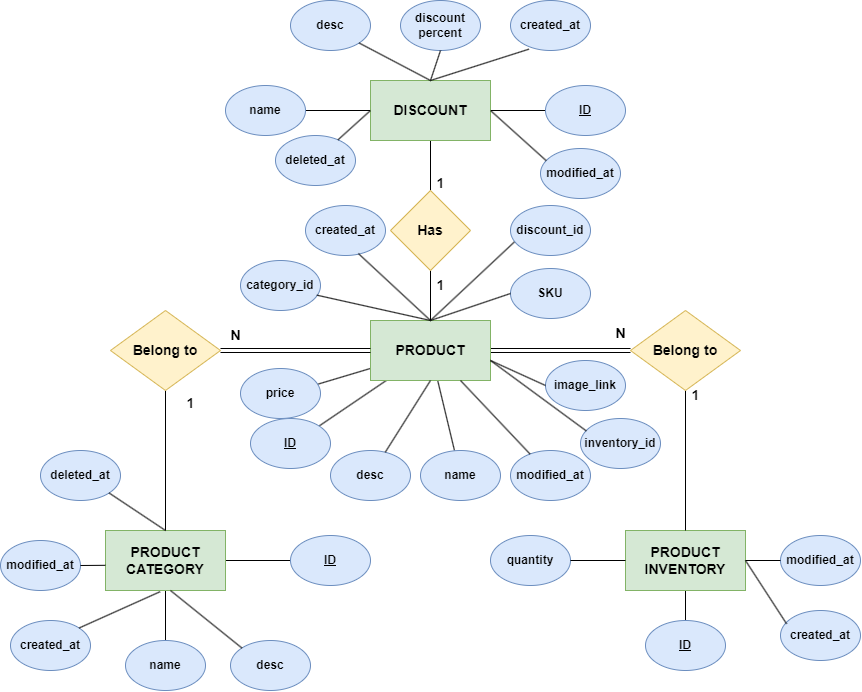
\includegraphics[scale=0.5]{images/hieu/chap-3/database-diagram.png}
    \caption{Entity Relationship Diagram - ERD}
\end{figure}
\subsubsection {Mô tả chi tiết thực thể}
\begin{itemize}
    \item \textbf{Product:} Thực thể này lưu trữ thông tin về sản phẩm của cửa hàng.
        \begin{table}[H]
        \begin{tabular}{|l|l|l|}
        \hline
        \textbf{Thuộc tính} & \textbf{Kiểu dữ liệu} & \textbf{Mô tả}                            \\ \hline
        ID                  & int                   & Mã sản phẩm - khoá chính                  \\ \hline
        name                & varchar               & Tên sản phẩm                              \\ \hline
        desc                & text                  & Mô tả sản phẩm                            \\ \hline
        SKU                 & varchar               & Kết hợp giữa mã sản phẩm và loại sản phẩm \\ \hline
        price               & decimal               & Giá của sản phẩm                          \\ \hline
        created\_at         & timestamp             & Thời gian tạo                             \\ \hline
        modified\_at        & timestamp             & Thời gian điều chỉnh                      \\ \hline
        image\_link         & string                & Liên kết chứa hỉnh ảnh sản phẩm           \\ \hline
        \end{tabular}
        \end{table}
    \item \textbf{Product Category:} Thực thể này lưu trữ thông tin về loại sản phẩm của cửa hàng.
            \begin{table}[H]
                \begin{tabular}{|l|l|l|}
                \hline
                \textbf{Thuộc tính} & \textbf{Kiểu dữ liệu} & \textbf{Mô tả}                \\ \hline
                ID                  & int                   & Mã loại sản phẩm - khoá chính \\ \hline
                name                & varchar               & Tên loại sản phẩm             \\ \hline
                desc                & text                  & Mô tả loại sản phẩm           \\ \hline
                deleted\_at         & timestamp             & Thời giản xoá loại sản phẩm   \\ \hline
                modified\_at        & timestamp             & Thời gian điều chỉnh          \\ \hline
                created\_at         & timestamp             & Thời gian tạo                 \\ \hline
                \end{tabular}
                \end{table}
    \item \textbf{Product Inventory:} Thực thể này lưu trữ thông tin về kho lưu trữ sản phẩm của cửa hàng.
        \begin{table}[H]
        \begin{tabular}{|l|l|l|}
        \hline
        \textbf{Thuộc tính} & \textbf{Kiểu dữ liệu} & \textbf{Mô tả}                \\ \hline
        ID                  & int                   & Mã loại sản phẩm - khoá chính \\ \hline
        quantity            & int                   & Số lượng sản phẩm             \\ \hline
        modified\_at        & timestamp             & Thời gian điều chỉnh          \\ \hline
        created\_at         & timestamp             & Thời gian tạo                 \\ \hline
        \end{tabular}
        \end{table}
    \item \textbf{Discount:} Thực thể này lưu trữ thông tin về khuyến mãi của sản phẩm.
        \begin{table}[H]
        \begin{tabular}{|l|l|l|}
        \hline
        \textbf{Thuộc tính} & \textbf{Kiểu dữ liệu} & \textbf{Mô tả}           \\ \hline
        ID                  & int                   & Mã giảm giá - khoá chính \\ \hline
        name                & varchar               & Tên giảm giá             \\ \hline
        desc                & text                  & Mô tả giảm giá           \\ \hline
        discount\_percent   & decimal               & Phần trăm giảm giá       \\ \hline
        created\_at         & timestamp             & Thời gian tạo            \\ \hline
        deleted\_at         & timestamp             & Thời gian xoá            \\ \hline
        Modified\_at        & timestamp             & Thời gian điều chỉnh     \\ \hline
        \end{tabular}
        \end{table}
\end{itemize}

\section{Phân tích bài toán và đề xuất giải pháp}

\subsection{Kết luận}
Từ việc phân tích các use case trên, chúng ta có thể rút ra được một số kết luận như sau:
\noindent Tất cả các use case đều sử dụng nền tảng cloud để xây dựng hệ thống nhằm đáp ứng tính 
scalability (khả năng mở rộng) và availability (tính sẵn sàng). Một số dịch vụ nền tảng cloud phổ biến nhất hiện nay để quản lý Kubernetes là EKS (Elastic Kubernetes Service) và AKS (Azure Kubernetes Service), các dịch vụ này có thể tự động hóa nhiều công việc và tích hợp tốt với các dịch vụ khác trong hệ sinh thái của nhà cung cấp đó nhằm giúp đơn giản hóa việc triển khai và quản lý cụm Kubernetes. \\[0.5cm]
Tuy nhiên, chúng ta có thể sử dụng Kubernetes để triển khai ứng dụng của mình trên bất kỳ nơi nào có hỗ trợ Kubernetes, mà không bị ràng buộc bởi một nhà cung cấp dịch vụ nào, hay nói cách khác nó độc lập với hạ tầng cụ thể. \\[0.5cm]
Bên cạnh đó, Kubernetes còn đảm bảo được hệ thống sẽ đáp ứng được tính scalability (khả năng mở rộng) và availability (tính sẵn sàng) thông qua một số dịch vụ và khái niệm của nó như:
\begin{itemize}
    \item ReplicaSets: Dùng để định nghĩa và duy trì một số lượng replicas (bản sao) của các pod chạy ứng dụng. Điều này giúp đảm bảo tính sẵn sàng của ứng dụng và có thể mở rộng hoặc thu hẹp số lượng replicas dựa trên tải công việc.
    \item Horizontal Pod Autoscaler (HPA): Cho phép tự động thay đổi số lượng replicas của một pod dựa trên các điều kiện như CPU và/hoặc bộ nhớ sử dụng.
    \item Cluster Autoscaler: Tự động mở rộng hoặc thu hẹp cụm Kubernetes bằng cách thêm hoặc giảm số lượng node dựa trên tải công việc.
    \item Load Balancer Services: Sử dụng để phân phối các yêu cầu đến các pod trong cụm, giúp đảm bảo tính sẵn sàng và chia tải đều.
    \item Readiness Probes: Cho phép Kubernetes kiểm tra tính sẵn sàng của mỗi pod trước khi chuyển lưu lượng truy cập đến nó.
    \item Liveness Probes: Kiểm tra xem một pod có hoạt động đúng cách hay không và tự động khởi động lại pod nếu cần.
    \item Pod Disruption Budgets: Giới hạn số lượng pods có thể bị tắt đồng thời trong khi thực hiện các cập nhật hoặc bảo trì để đảm bảo tính sẵn sàng.
\end{itemize}
\noindent Đa phần kiến trúc microservice được ưu tiên áp dụng vì đây là một mô hình ít phụ thuộc vào nhau nên chúng có thể được triển khai, quản lý và mở rộng độc lập với nhau, đồng thời cũng giảm áp lực cho hệ thống vì chúng không cần phải tương tác trực tiếp với nhau mà thông qua message queue (Apache Kafka, RabbitMQ, ActiveMQ, và Microsoft Azure Service Bus).
\subsection{Đề xuất giải pháp}
\noindent Từ các phân tích và kết luận ở trên, nhóm quyết định sẽ xây dựng hệ thống dưới dạng microservice và deloy ứng dụng bằng Kubernetes. Với Kubernetes, ứng dụng sẽ đáp ứng được tính mở rộng và tính sẵn sàng cao thông qua một số dịch vụ mà Kubernetes cung cấp: deloyment, HPA, masternode v.v. Các service của hệ thống sẽ giao tiếp với nhau thông qua message queue.
\chapter{Thiết kế hệ thống}
\section{Thiết kế giao diện bằng ứng dụng Figma}
\subsection{Thiết kế giao diện trang hiển thị sản phẩm}
\begin{figure}[H]
    \begin{center}
    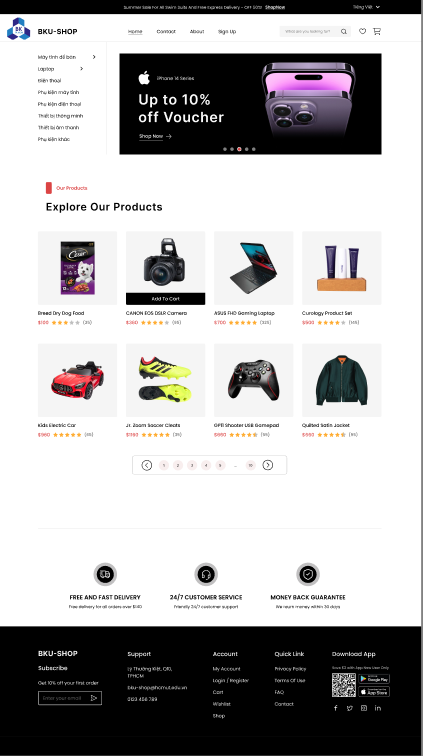
\includegraphics[scale=0.8]{images/hieu/chap-4/display-product-page.png}
    \vspace*{5mm}
    \caption{Thiêt kế giao diện trang hiển thị sản phẩm}
    \end{center}
\end{figure}
\begin{itemize}
    \item \textbf{Phần Header}
    \newline
    Phần đầu trang web gồm các thành phần sau:
    \begin{itemize}
        \item Logo của trang web
        \item Tên trang web
        \item Thanh điều hướng chứa các nút điều hướng đến các trang khác
        \item Ô tìm kiếm sản phẩm
        \item Nút đăng nhập
        \item Giỏ hàng
    \end{itemize}
    \begin{figure}[H]
        \begin{center}
        
\includegraphics[scale=0.5]{images/hieu/chap-4/header.png}
        \vspace*{5mm}
        \caption{Phần đầu trang - Header}
        \end{center}
    \end{figure}

    \item \textbf{Phần Category}
    \newline
    Phần category là một thanh dropdown chứa các danh mục sản phẩm.
    \begin{figure}[H]
        \begin{center}
        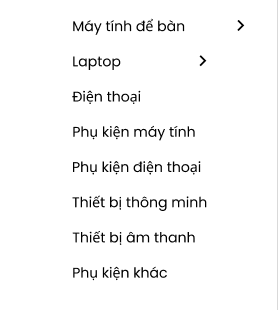
\includegraphics[scale=1]{images/hieu/chap-4/category.png}
        \vspace*{5mm}
        \caption{Phần danh mục sản phẩm - Category}
        \end{center}
    \end{figure}
    \item \textbf{Phần Discount}
    \newline
    Phần discount là một slide chứa các giảm giá của các sản phẩm. Slide sẽ tự chuyển động sau một khoảng thời gian nhất định hoặc có thể chuyển động bằng cách nhấn vào các nút điều hướng.
    \begin{figure}[H]
        \begin{center}
        
\includegraphics[scale=0.7]{images/hieu/chap-4/discount.png}
        \vspace*{5mm}
        \caption{Phần giảm giá - Discount}
        \end{center}
    \end{figure}
    \item \textbf{Phần Product}
    \newline
    Phần product hiển thị các sản phẩm theo danh mục. Mỗi sản phẩm gồm có:
    \begin{itemize}
        \item Hình ảnh sản phẩm
        \item Tên sản phẩm
        \item Giá sản phẩm
        \item Nút thêm vào giỏ hàng
        \item Nút xem chi tiết sản phẩm
    \end{itemize}
    \begin{figure}[H]
        \begin{center}
        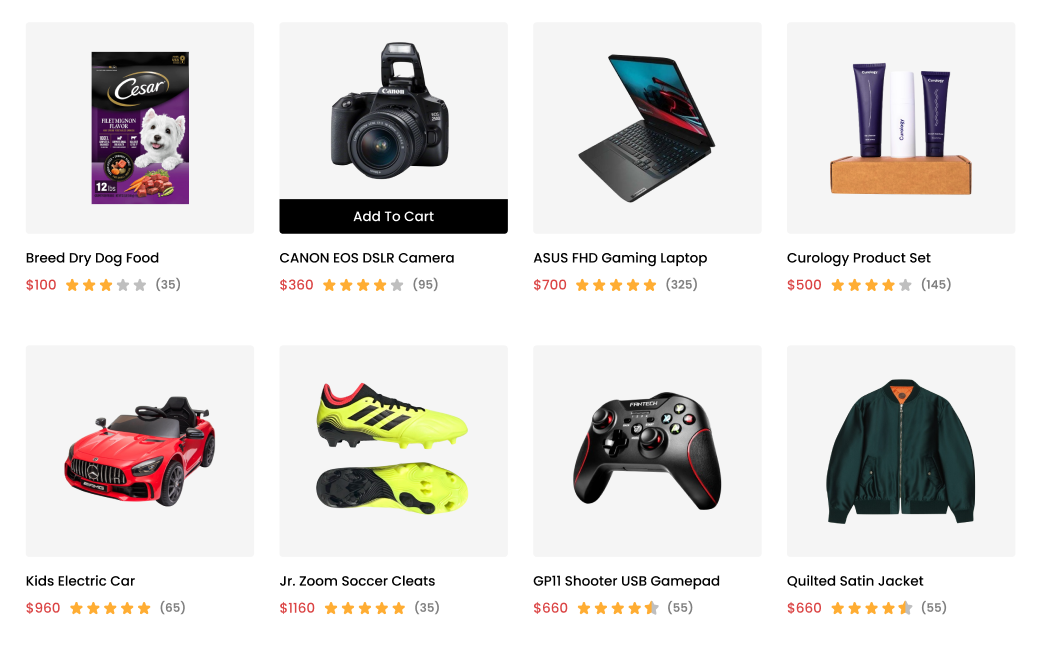
\includegraphics[scale=0.7]{images/hieu/chap-4/product.png}
        \vspace*{5mm}
        \caption{Phần sản phẩm - Product}
        \end{center}
    \end{figure}
    \item \textbf{Phần Footer}
    \newline
    Phần footer là phần cuối trang web chứa các thông tin về trang web, các liên kết đến các trang mạng xã hội, các liên kết đến các trang khác.
    \begin{figure}[H]
        \begin{center}
        
\includegraphics[scale=0.5]{images/hieu/chap-4/footer.png}
        \vspace*{5mm}
        \caption{Phần cuối trang - Footer}
        \end{center}
    \end{figure}
\end{itemize}
\chapter{Xây dựng phiên bản thử nghiệm}
% \input{sections/chapter6}
\chapter{Tổng kết}
% \input{sections/conclusion}
% \cleardoublepage
\phantomsection
\addcontentsline{toc}{chapter}{Tài liệu tham khảo}

\begin{thebibliography}{1}

\bibitem {react}
Meta Platforms Inc (2023), \emph{React Tutorial}, URL: \url{https://reactjs.org/}, truy cập lần cuối: 17/12/2023.

\bibitem{springboot}
LTS EDU (2023), \emph{Java Spring Boot là gì ? Java Spring MVC là gì ? Spring Framework là gì ?}, URL: \url{https://lotusacademy.edu.vn/blog/java-spring-boot-la-gi-java-spring-mvc-la-gi-spring-framework-la-gi-256}, truy cập lần cuối: 17/12/2023.

\bibitem{nodejs}
NodeJS (2023), \emph{About Node.js}, URL: \url{https://nodejs.org/en/about}, truy cập lần cuối: 17/12/2023.

\bibitem{docker}
Docker (2023), \emph{Docker docs}, URL: \url{https://docs.docker.com/}, truy cập lần cuối: 17/12/2023.

\bibitem{postgres}
PostgreSQL (2023), \emph{PostgreSQL: The World's Most Advanced Open Source Relational Database}, URL: \url{https://www.postgresql.org/}, truy cập lần cuối: 17/12/2023.

\bibitem{terraform}
Terraform by HashiCorp (2023), \emph{Terraform Docs}, URL: \url{https://developer.hashicorp.com/terraform?product_intent=terraform}, truy cập lần cuối: 17/12/2023.

\bibitem{terraform_2}
Tran Phuc Hau (23/4/2023), \emph{Terraform là gì?}, URL: \url{https://www.alibabacloud.com/blog/terraform-l%C3%A0-g%C3%AC-_599921}, truy cập lần cuối: 17/12/2023.

\bibitem{k8s}
Kubernetes - Tài liệu (2023), \emph{Kubernetes là gì}, URL: \url{https://kubernetes.io/vi/docs/concepts/overview/what-is-kubernetes}, truy cập lần cuối: 17/12/2023.

\bibitem{eks}
AWS (2023), \emph{Dịch vụ Kubernetes linh hoạt Amazon}, URL: \url{https://aws.amazon.com/vi/eks/}, truy cập lần cuối: 17/12/2023.

\bibitem{aks}
Microsoft Learn (2023), \emph{What is Azure Kubernetes Service?}, URL: \url{https://learn.microsoft.com/en-us/azure/aks/intro-kubernetes}, truy cập lần cuối: 17/12/2023.

\bibitem{rabbitmq}
Gabor Olah, \emph{An introduction to RabbitMQ - What is RabbitMQ?}, URL: \url{https://www.erlang-solutions.com/blog/an-introduction-to-rabbitmq-what-is-rabbitmq/}, truy cập lần cuối: 17/12/2023.

\bibitem{availability_n_scalability}
Microsoft Learn (2023), \emph{Describe the benefits of high availability and scalability in the cloud}, URL: \url{https://learn.microsoft.com/en-us/training/modules/describe-benefits-use-cloud-services/2-high-availability-scalability-cloud}, truy cập lần cuối: 17/12/2023.

\bibitem{mono_vs_ms}
Microsoft Learn (2023), \emph{Decompose a monolithic application into a microservices architecture}, URL: \url{https://learn.microsoft.com/en-us/training/modules/microservices-architecture/}, truy cập lần cuối 17/12/2023.

\bibitem{case_aks_1}
Microsoft Learn (2023), \emph{Microservices architecture on Azure Kubernetes Service}, URL: \url{https://learn.microsoft.com/en-us/azure/architecture/reference-architectures/containers/aks-microservices/aks-microservices}, truy cập lần cuối 17/12/2023.


\bibitem{case_aks_2}
Microsoft Learn (2023), \emph{Advanced Azure Kubernetes Service (AKS) microservices architecture}, URL: \url{https://learn.microsoft.com/en-us/azure/architecture/reference-architectures/containers/aks-microservices/aks-microservices-advanced/}, truy cập lần cuối 17/12/2023.

\bibitem{case_aks_3}
Microsoft Learn (2023), \emph{Magento e-commerce platform in Azure Kubernetes Service}, URL: \url{https://learn.microsoft.com/en-us/azure/architecture/example-scenario/magento/magento-azure}, truy cập lần cuối 17/12/2023.

\bibitem{case_aws_1}
Saurabh Shrivastava (16/01/2018), \emph{Scale Your Web Application — One Step at a Time}, URL: \url{https://aws.amazon.com/vi/blogs/architecture/scale-your-web-application-one-step-at-a-time/}, truy cập lần cuối 17/12/2023.

\bibitem{case_aws_2}
Adritano Cataluddi (08/02/2023), \emph{Scaling PHP Applications on AWS}, URL: \url{https://www.logicata.com/blog/scaling-php-applications-on-aws/}, truy cập lần cuối 17/12/2023.

\bibitem{case_aws_3}
Stacksimplify (2023), \emph{Microservices Deployment on EKS}, URL: \url{https://www.stacksimplify.com/aws-eks/microservices-on-aws-eks/learn-to-deploy-microservices-on-aws-eks/}, truy cập lần cuối 17/12/2023.

\bibitem{minikube}
Minikube (2023), \emph{Documentation}, URL: \url{https://minikube.sigs.k8s.io/docs/}, truy cập lần cuối 17/12/2023.


\end{thebibliography}
% \input{sections/appendixes}
% \input{sections/task_division}

\endgroup



\end{document}